\documentclass[]{article}
\usepackage{lmodern}
\usepackage{setspace}
\setstretch{1}
\usepackage{amssymb,amsmath}
\usepackage{ifxetex,ifluatex}
\usepackage{fixltx2e} % provides \textsubscript
\ifnum 0\ifxetex 1\fi\ifluatex 1\fi=0 % if pdftex
  \usepackage[T1]{fontenc}
  \usepackage[utf8]{inputenc}
\else % if luatex or xelatex
  \ifxetex
    \usepackage{mathspec}
  \else
    \usepackage{fontspec}
  \fi
  \defaultfontfeatures{Ligatures=TeX,Scale=MatchLowercase}
\fi
% use upquote if available, for straight quotes in verbatim environments
\IfFileExists{upquote.sty}{\usepackage{upquote}}{}
% use microtype if available
\IfFileExists{microtype.sty}{%
\usepackage{microtype}
\UseMicrotypeSet[protrusion]{basicmath} % disable protrusion for tt fonts
}{}
\usepackage[margin=1in]{geometry}
\usepackage{hyperref}
\PassOptionsToPackage{usenames,dvipsnames}{color} % color is loaded by hyperref
\hypersetup{unicode=true,
            pdftitle={Component response rate variation underlies the stability of complex systems},
            pdfauthor={A. Bradley Duthie},
            colorlinks=true,
            linkcolor=blue,
            citecolor=Blue,
            urlcolor=Blue,
            breaklinks=true}
\urlstyle{same}  % don't use monospace font for urls
\usepackage{color}
\usepackage{fancyvrb}
\newcommand{\VerbBar}{|}
\newcommand{\VERB}{\Verb[commandchars=\\\{\}]}
\DefineVerbatimEnvironment{Highlighting}{Verbatim}{commandchars=\\\{\}}
% Add ',fontsize=\small' for more characters per line
\usepackage{framed}
\definecolor{shadecolor}{RGB}{248,248,248}
\newenvironment{Shaded}{\begin{snugshade}}{\end{snugshade}}
\newcommand{\KeywordTok}[1]{\textcolor[rgb]{0.13,0.29,0.53}{\textbf{#1}}}
\newcommand{\DataTypeTok}[1]{\textcolor[rgb]{0.13,0.29,0.53}{#1}}
\newcommand{\DecValTok}[1]{\textcolor[rgb]{0.00,0.00,0.81}{#1}}
\newcommand{\BaseNTok}[1]{\textcolor[rgb]{0.00,0.00,0.81}{#1}}
\newcommand{\FloatTok}[1]{\textcolor[rgb]{0.00,0.00,0.81}{#1}}
\newcommand{\ConstantTok}[1]{\textcolor[rgb]{0.00,0.00,0.00}{#1}}
\newcommand{\CharTok}[1]{\textcolor[rgb]{0.31,0.60,0.02}{#1}}
\newcommand{\SpecialCharTok}[1]{\textcolor[rgb]{0.00,0.00,0.00}{#1}}
\newcommand{\StringTok}[1]{\textcolor[rgb]{0.31,0.60,0.02}{#1}}
\newcommand{\VerbatimStringTok}[1]{\textcolor[rgb]{0.31,0.60,0.02}{#1}}
\newcommand{\SpecialStringTok}[1]{\textcolor[rgb]{0.31,0.60,0.02}{#1}}
\newcommand{\ImportTok}[1]{#1}
\newcommand{\CommentTok}[1]{\textcolor[rgb]{0.56,0.35,0.01}{\textit{#1}}}
\newcommand{\DocumentationTok}[1]{\textcolor[rgb]{0.56,0.35,0.01}{\textbf{\textit{#1}}}}
\newcommand{\AnnotationTok}[1]{\textcolor[rgb]{0.56,0.35,0.01}{\textbf{\textit{#1}}}}
\newcommand{\CommentVarTok}[1]{\textcolor[rgb]{0.56,0.35,0.01}{\textbf{\textit{#1}}}}
\newcommand{\OtherTok}[1]{\textcolor[rgb]{0.56,0.35,0.01}{#1}}
\newcommand{\FunctionTok}[1]{\textcolor[rgb]{0.00,0.00,0.00}{#1}}
\newcommand{\VariableTok}[1]{\textcolor[rgb]{0.00,0.00,0.00}{#1}}
\newcommand{\ControlFlowTok}[1]{\textcolor[rgb]{0.13,0.29,0.53}{\textbf{#1}}}
\newcommand{\OperatorTok}[1]{\textcolor[rgb]{0.81,0.36,0.00}{\textbf{#1}}}
\newcommand{\BuiltInTok}[1]{#1}
\newcommand{\ExtensionTok}[1]{#1}
\newcommand{\PreprocessorTok}[1]{\textcolor[rgb]{0.56,0.35,0.01}{\textit{#1}}}
\newcommand{\AttributeTok}[1]{\textcolor[rgb]{0.77,0.63,0.00}{#1}}
\newcommand{\RegionMarkerTok}[1]{#1}
\newcommand{\InformationTok}[1]{\textcolor[rgb]{0.56,0.35,0.01}{\textbf{\textit{#1}}}}
\newcommand{\WarningTok}[1]{\textcolor[rgb]{0.56,0.35,0.01}{\textbf{\textit{#1}}}}
\newcommand{\AlertTok}[1]{\textcolor[rgb]{0.94,0.16,0.16}{#1}}
\newcommand{\ErrorTok}[1]{\textcolor[rgb]{0.64,0.00,0.00}{\textbf{#1}}}
\newcommand{\NormalTok}[1]{#1}
\usepackage{longtable,booktabs}
\usepackage{graphicx,grffile}
\makeatletter
\def\maxwidth{\ifdim\Gin@nat@width>\linewidth\linewidth\else\Gin@nat@width\fi}
\def\maxheight{\ifdim\Gin@nat@height>\textheight\textheight\else\Gin@nat@height\fi}
\makeatother
% Scale images if necessary, so that they will not overflow the page
% margins by default, and it is still possible to overwrite the defaults
% using explicit options in \includegraphics[width, height, ...]{}
\setkeys{Gin}{width=\maxwidth,height=\maxheight,keepaspectratio}
\IfFileExists{parskip.sty}{%
\usepackage{parskip}
}{% else
\setlength{\parindent}{0pt}
\setlength{\parskip}{6pt plus 2pt minus 1pt}
}
\setlength{\emergencystretch}{3em}  % prevent overfull lines
\providecommand{\tightlist}{%
  \setlength{\itemsep}{0pt}\setlength{\parskip}{0pt}}
\setcounter{secnumdepth}{0}
% Redefines (sub)paragraphs to behave more like sections
\ifx\paragraph\undefined\else
\let\oldparagraph\paragraph
\renewcommand{\paragraph}[1]{\oldparagraph{#1}\mbox{}}
\fi
\ifx\subparagraph\undefined\else
\let\oldsubparagraph\subparagraph
\renewcommand{\subparagraph}[1]{\oldsubparagraph{#1}\mbox{}}
\fi

%%% Use protect on footnotes to avoid problems with footnotes in titles
\let\rmarkdownfootnote\footnote%
\def\footnote{\protect\rmarkdownfootnote}

%%% Change title format to be more compact
\usepackage{titling}

% Create subtitle command for use in maketitle
\newcommand{\subtitle}[1]{
  \posttitle{
    \begin{center}\large#1\end{center}
    }
}

\setlength{\droptitle}{-2em}

  \title{Component response rate variation underlies the stability of complex
systems}
    \pretitle{\vspace{\droptitle}\centering\huge}
  \posttitle{\par}
  \subtitle{Supplemental Information}
  \author{A. Bradley Duthie}
    \preauthor{\centering\large\emph}
  \postauthor{\par}
      \predate{\centering\large\emph}
  \postdate{\par}
    \date{Biological and Environmental Sciences, University of Stirling, Stirling,
UK, FK9 4LA
\href{mailto:alexander.duthie@stir.ac.uk}{\nolinkurl{alexander.duthie@stir.ac.uk}}}

\usepackage{amsmath}
\usepackage{natbib}
\usepackage{lineno}
\usepackage[utf8]{inputenc}
\usepackage{float}
\linenumbers
\bibliographystyle{amnatnat}

\begin{document}
\maketitle

\begin{center}\rule{0.5\linewidth}{\linethickness}\end{center}

\textbf{This supplemental information supports the manuscript
``Component response rate variation drives stability in large complex
systems'' with additional analyses to support its conclusions. All text,
code, and data underlying this manuscript are publicly available on
\href{https://github.com/bradduthie/RandomMatrixStability}{GitHub} as
part of the RandomMatrixStability R package.}

The
\href{https://github.com/bradduthie/RandomMatrixStability}{RandomMatrixStability
package} includes all functions and tools for recreating the text, this
supplemental information, and running all code; additional documentation
is also provided for package functions. The RandomMatrixStability
package is available on
\href{https://github.com/bradduthie/RandomMatrixStability}{GitHub}; to
download it, the
\href{https://cran.r-project.org/web/packages/devtools/index.html}{\texttt{devtools}
library} is needed.

\begin{Shaded}
\begin{Highlighting}[]
\KeywordTok{install.packages}\NormalTok{(}\StringTok{"devtools"}\NormalTok{);}
\KeywordTok{library}\NormalTok{(devtools);}
\end{Highlighting}
\end{Shaded}

The code below installs the RandomMatrixStability package using
devtools.

\begin{Shaded}
\begin{Highlighting}[]
\KeywordTok{install_github}\NormalTok{(}\StringTok{"bradduthie/RandomMatrixStability"}\NormalTok{);}
\end{Highlighting}
\end{Shaded}

\begin{center}\rule{0.5\linewidth}{\linethickness}\end{center}

\section{Supplemental Information table of
contents}\label{supplemental-information-table-of-contents}

\begin{itemize}
\tightlist
\item
  \protect\hyperlink{IncrS}{Stability across increasing \(S\)}
\item
  \protect\hyperlink{ecological}{Stability of ecological networks}

  \begin{itemize}
  \tightlist
  \item
    \protect\hyperlink{competition}{Competitor networks}
  \item
    \protect\hyperlink{mutualism}{Mutualist networks}
  \item
    \protect\hyperlink{pred-prey}{Predator-prey networks}
  \end{itemize}
\item
  \protect\hyperlink{connectance}{Sensitivity of connectance (C) values}

  \begin{itemize}
  \tightlist
  \item
    \protect\hyperlink{connect3}{C = 0.3}
  \item
    \protect\hyperlink{connect5}{C = 0.5}
  \item
    \protect\hyperlink{connect7}{C = 0.7}
  \item
    \protect\hyperlink{connect9}{C = 0.9}
  \end{itemize}
\item
  \protect\hyperlink{sigma}{Large networks of \(C = 0.05\) across \(S\)
  and \(\sigma\)}

  \begin{itemize}
  \tightlist
  \item
    \protect\hyperlink{sigma3}{\(\sigma\) = 0.3}
  \item
    \protect\hyperlink{sigma4}{\(\sigma\) = 0.4}
  \item
    \protect\hyperlink{sigma5}{\(\sigma\) = 0.5}
  \item
    \protect\hyperlink{sigma6}{\(\sigma\) = 0.6}
  \end{itemize}
\item
  \protect\hyperlink{gam_dist}{Sensitivity of distribution of
  \(\gamma\)}
\item
  \protect\hyperlink{Feasibility}{Feasibility of complex systems}
\item
  \protect\hyperlink{ga}{Stability given targeted manipulation of
  \(\gamma\) (genetic algorithm)}
\item
  \protect\hyperlink{Gibbs}{Consistency with Gibbs et al. (2018)}
\item
  \protect\hyperlink{rhos}{Effects of matrix correlations}
\end{itemize}

\hypertarget{IncrS}{\section{\texorpdfstring{Stability across increasing
\(S\)}{Stability across increasing S}}\label{IncrS}}

Figure 4 of the main text reports the number of stable random complex
systems found over 1 million iterations. The table below shows the
results for all simulations of random \(\mathbf{M}\) matrices at
\(\sigma = 0.4\) and \(C = 1\) given a range of
\(S = \{2, 3, ..., 49, 50\}\). In this table, the \texttt{A0} refers to
matrices where \(\gamma = 1\), while \texttt{A1} refers to matrices
after \(Var(\gamma)\) is added and \(\gamma \sim \mathcal{U}(0, 2)\).
Each row summarises data for a given \(S\) over 1 million randomly
simulated \(\mathbf{M}\) (\texttt{A0} and \texttt{A1}). The column
\texttt{A0\_unstable} shows the number of \texttt{A0} matrices that are
unstable, and the column \texttt{A0\_stable} shows the number of
\texttt{A0} matrices that are stable (these two columns sum to 1
million). Similarly, the column \texttt{A1\_unstable} shows the number
of \texttt{A1} matrices that are unstable and \texttt{A1\_stable} shows
the number that are stable. The columns \texttt{A1\_stabilised} and
\texttt{A1\_destabilised} show how many \texttt{A0} matrices were
stabilised or destabilised, respectively, by \(Var(\gamma)\).

\begin{longtable}[]{@{}rrrrrrr@{}}
\toprule
S & A0\_unstable & A0\_stable & A1\_unstable & A1\_stable &
A1\_stabilised & A1\_destabilised\tabularnewline
\midrule
\endhead
2 & 293 & 999707 & 293 & 999707 & 0 & 0\tabularnewline
3 & 3602 & 996398 & 3609 & 996391 & 0 & 7\tabularnewline
4 & 14937 & 985063 & 15008 & 984992 & 0 & 71\tabularnewline
5 & 39289 & 960711 & 39783 & 960217 & 36 & 530\tabularnewline
6 & 78845 & 921155 & 80207 & 919793 & 389 & 1751\tabularnewline
7 & 133764 & 866236 & 136904 & 863096 & 1679 & 4819\tabularnewline
8 & 204112 & 795888 & 208241 & 791759 & 5391 & 9520\tabularnewline
9 & 288041 & 711959 & 291775 & 708225 & 12619 & 16353\tabularnewline
10 & 384024 & 615976 & 384931 & 615069 & 23153 & 24060\tabularnewline
11 & 485975 & 514025 & 481019 & 518981 & 35681 & 30725\tabularnewline
12 & 590453 & 409547 & 577439 & 422561 & 48302 & 35288\tabularnewline
13 & 689643 & 310357 & 669440 & 330560 & 57194 & 36991\tabularnewline
14 & 777496 & 222504 & 751433 & 248567 & 60959 & 34896\tabularnewline
15 & 850159 & 149841 & 821613 & 178387 & 58567 & 30021\tabularnewline
16 & 905057 & 94943 & 877481 & 122519 & 51255 & 23679\tabularnewline
17 & 943192 & 56808 & 919536 & 80464 & 40854 & 17198\tabularnewline
18 & 969018 & 30982 & 949944 & 50056 & 30102 & 11028\tabularnewline
19 & 984301 & 15699 & 970703 & 29297 & 20065 & 6467\tabularnewline
20 & 992601 & 7399 & 983507 & 16493 & 12587 & 3493\tabularnewline
21 & 996765 & 3235 & 991532 & 8468 & 7030 & 1797\tabularnewline
22 & 998693 & 1307 & 995567 & 4433 & 3884 & 758\tabularnewline
23 & 999503 & 497 & 997941 & 2059 & 1883 & 321\tabularnewline
24 & 999861 & 139 & 999059 & 941 & 899 & 97\tabularnewline
25 & 999964 & 36 & 999617 & 383 & 380 & 33\tabularnewline
26 & 999993 & 7 & 999878 & 122 & 121 & 6\tabularnewline
27 & 999995 & 5 & 999946 & 54 & 53 & 4\tabularnewline
28 & 1000000 & 0 & 999975 & 25 & 25 & 0\tabularnewline
29 & 1000000 & 0 & 999997 & 3 & 3 & 0\tabularnewline
30 & 1000000 & 0 & 999999 & 1 & 1 & 0\tabularnewline
31 & 1000000 & 0 & 999999 & 1 & 1 & 0\tabularnewline
32 & 1000000 & 0 & 1000000 & 0 & 0 & 0\tabularnewline
33 & 1000000 & 0 & 1000000 & 0 & 0 & 0\tabularnewline
34 & 1000000 & 0 & 1000000 & 0 & 0 & 0\tabularnewline
35 & 1000000 & 0 & 1000000 & 0 & 0 & 0\tabularnewline
36 & 1000000 & 0 & 1000000 & 0 & 0 & 0\tabularnewline
37 & 1000000 & 0 & 1000000 & 0 & 0 & 0\tabularnewline
38 & 1000000 & 0 & 1000000 & 0 & 0 & 0\tabularnewline
39 & 1000000 & 0 & 1000000 & 0 & 0 & 0\tabularnewline
40 & 1000000 & 0 & 1000000 & 0 & 0 & 0\tabularnewline
41 & 1000000 & 0 & 1000000 & 0 & 0 & 0\tabularnewline
42 & 1000000 & 0 & 1000000 & 0 & 0 & 0\tabularnewline
43 & 1000000 & 0 & 1000000 & 0 & 0 & 0\tabularnewline
44 & 1000000 & 0 & 1000000 & 0 & 0 & 0\tabularnewline
45 & 1000000 & 0 & 1000000 & 0 & 0 & 0\tabularnewline
46 & 1000000 & 0 & 1000000 & 0 & 0 & 0\tabularnewline
47 & 1000000 & 0 & 1000000 & 0 & 0 & 0\tabularnewline
48 & 1000000 & 0 & 1000000 & 0 & 0 & 0\tabularnewline
49 & 1000000 & 0 & 1000000 & 0 & 0 & 0\tabularnewline
50 & 1000000 & 0 & 1000000 & 0 & 0 & 0\tabularnewline
\bottomrule
\end{longtable}

Overall, the ratio of stable \texttt{A1} matrices to stable \texttt{A0}
matrices found is greater than 1 whenever \(S > 10\) (compare column 5
to column 3), and this ratio increases with increasing \(S\) (column 1).
Hence, more randomly created complex systems (\(\mathbf{M}\)) are stable
given variation in \(\gamma\) than when \(\gamma = 1\). Note that
feasibility results were omitted for the table above, but are
\protect\hyperlink{Feasibility}{reported below}.

\hypertarget{ecological}{\section{Stability of ecological
networks}\label{ecological}}

While the foundational work of
May\textsuperscript{\protect\hyperlink{ref-May1972}{1}} applies broadly
to complex networks, much attention has been given specifically to
ecological networks of interacting species. In these networks, the
matrix \(\mathbf{A}\) is interpreted as a community matrix and each row
and column is interpreted as a single species. The per capita effect
that the density of any species \(i\) has on the population dynamics of
species \(j\) is found in \(A_{ij}\), meaning that \(\mathbf{A}\) holds
the effects of pair-wise interactions between \(S\)
species\textsuperscript{\protect\hyperlink{ref-Allesina2012}{2},\protect\hyperlink{ref-Allesina2015}{3}}.
While May's original
work\textsuperscript{\protect\hyperlink{ref-May1972}{1}} considered only
randomly assembled communities, recent work has specifically looked at
more restricted ecological communities including competitive networks
(all off-diagonal elements of \(\mathbf{A}\) are negative), mutualist
networks (all off-diagonal elements of \(\mathbf{A}\) are positive), and
predator-prey networks (for any pair of \(i\) and \(j\), the effect of
\(i\) on \(j\) is negative and \(j\) on \(i\) is positive, or vice
versa)\textsuperscript{\protect\hyperlink{ref-Allesina2012}{2},\protect\hyperlink{ref-Allesina2015}{3}}.
In general, competitor and mutualist networks tend to be unstable, while
predator-prey networks tend to be highly
stabilising\textsuperscript{\protect\hyperlink{ref-Allesina2012}{2}}.

I investigated competitor, mutualist, and predator-prey networks
following Allesina et
al.\textsuperscript{\protect\hyperlink{ref-Allesina2012}{2}}. To create
these networks, I first generated a random matrix \(\mathbf{A}\), then
changed the elements of \(\mathbf{A}\) accordingly. If \(\mathbf{A}\)
was a competitive network, then the sign of any positive off-diagonal
elements was reversed to be negative. If \(\mathbf{A}\) was a mutualist
network, then the sign of any positive off-diagonal elements was
reversed to be positive. And if \(\mathbf{A}\) was a predator-prey
network, then all \(i\) and \(j\) pairs of elements were checked; any
pairs of the same sign were changed so that one was negative and the
other was positive.

The number of stable \(\mathbf{M = \gamma A}\) systems was estimated
\protect\hyperlink{IncrS}{exactly as it was} in the main text for random
matrices for values of \(S\) from 2 to 50 (100 in the case of the
relatively more stable predator-prey interactions), except that only
100000 random \(\mathbf{M}\) were generated instead of 1 million.

The following tables for restricted ecological communities can therefore
be compared with the random \(\mathbf{M}\)
\protect\hyperlink{IncrS}{results above} (but note that counts from
systems with comparable probabilities of stability will be an order of
magnitude lower in the tables below due to the smaller number of
\(\mathbf{M}\) matrices generated). As with the
\protect\hyperlink{IncrS}{results above}, in the tables below,
\texttt{A0} refers to matrices when \(\gamma = 1\) and \texttt{A1}
refers to matrices after \(Var(\gamma)\) is added. The column
\texttt{A0\_unstable} shows the number of \texttt{A0} matrices that are
unstable, and the column \texttt{A0\_stable} shows the number of
\texttt{A0} matrices that are stable (these two columns sum to 100000).
Similarly, the column \texttt{A1\_unstable} shows the number of
\texttt{A1} matrices that are unstable and \texttt{A1\_stable} shows the
number that are stable. The columns \texttt{A1\_stabilised} and
\texttt{A1\_destabilised} show how many \texttt{A0} matrices were
stabilised or destabilised, respectively, by \(Var(\gamma)\).

\textbf{Competition}

Results for competitor interaction networks are shown below

\begin{longtable}[]{@{}lllllll@{}}
\toprule
N & A0\_unstable & A0\_stable & A1\_unstable & A1\_stable &
A1\_stabilised & A1\_destabilised\tabularnewline
\midrule
\endhead
2 & 48 & 99952 & 48 & 99952 & 0 & 0\tabularnewline
3 & 229 & 99771 & 231 & 99769 & 0 & 2\tabularnewline
4 & 701 & 99299 & 704 & 99296 & 0 & 3\tabularnewline
5 & 1579 & 98421 & 1587 & 98413 & 0 & 8\tabularnewline
6 & 3218 & 96782 & 3253 & 96747 & 6 & 41\tabularnewline
7 & 5519 & 94481 & 5619 & 94381 & 23 & 123\tabularnewline
8 & 9062 & 90938 & 9237 & 90763 & 77 & 252\tabularnewline
9 & 13436 & 86564 & 13729 & 86271 & 230 & 523\tabularnewline
10 & 18911 & 81089 & 19303 & 80697 & 505 & 897\tabularnewline
11 & 25594 & 74406 & 25961 & 74039 & 1011 & 1378\tabularnewline
12 & 33207 & 66793 & 33382 & 66618 & 1724 & 1899\tabularnewline
13 & 41160 & 58840 & 41089 & 58911 & 2655 & 2584\tabularnewline
14 & 50575 & 49425 & 49894 & 50106 & 3777 & 3096\tabularnewline
15 & 59250 & 40750 & 57892 & 42108 & 4824 & 3466\tabularnewline
16 & 67811 & 32189 & 65740 & 34260 & 5634 & 3563\tabularnewline
17 & 75483 & 24517 & 73056 & 26944 & 5943 & 3516\tabularnewline
18 & 82551 & 17449 & 79878 & 20122 & 5780 & 3107\tabularnewline
19 & 88030 & 11970 & 85204 & 14796 & 5417 & 2591\tabularnewline
20 & 92254 & 7746 & 89766 & 10234 & 4544 & 2056\tabularnewline
21 & 95233 & 4767 & 93002 & 6998 & 3695 & 1464\tabularnewline
22 & 97317 & 2683 & 95451 & 4549 & 2803 & 937\tabularnewline
23 & 98508 & 1492 & 97122 & 2878 & 1991 & 605\tabularnewline
24 & 99240 & 760 & 98407 & 1593 & 1216 & 383\tabularnewline
25 & 99669 & 331 & 99082 & 918 & 739 & 152\tabularnewline
26 & 99871 & 129 & 99490 & 510 & 452 & 71\tabularnewline
27 & 99938 & 62 & 99732 & 268 & 240 & 34\tabularnewline
28 & 99985 & 15 & 99888 & 112 & 108 & 11\tabularnewline
29 & 99990 & 10 & 99951 & 49 & 46 & 7\tabularnewline
30 & 100000 & 0 & 99981 & 19 & 19 & 0\tabularnewline
31 & 100000 & 0 & 99993 & 7 & 7 & 0\tabularnewline
32 & 100000 & 0 & 99996 & 4 & 4 & 0\tabularnewline
33 & 100000 & 0 & 99998 & 2 & 2 & 0\tabularnewline
34 & 100000 & 0 & 100000 & 0 & 0 & 0\tabularnewline
\ldots{} & \ldots{} & \ldots{} & \ldots{} & \ldots{} & \ldots{} &
\ldots{}\tabularnewline
50 & 100000 & 0 & 100000 & 0 & 0 & 0\tabularnewline
\bottomrule
\end{longtable}

\textbf{Mutualism}

Results for mutualist interaction networks are shown below

\begin{longtable}[]{@{}lllllll@{}}
\toprule
N & A0\_unstable & A0\_stable & A1\_unstable & A1\_stable &
A1\_stabilised & A1\_destabilised\tabularnewline
\midrule
\endhead
2 & 56 & 99944 & 56 & 99944 & 0 & 0\tabularnewline
3 & 3301 & 96699 & 3301 & 96699 & 0 & 0\tabularnewline
4 & 34446 & 65554 & 34446 & 65554 & 0 & 0\tabularnewline
5 & 86520 & 13480 & 86520 & 13480 & 0 & 0\tabularnewline
6 & 99683 & 317 & 99683 & 317 & 0 & 0\tabularnewline
7 & 99998 & 2 & 99998 & 2 & 0 & 0\tabularnewline
8 & 100000 & 0 & 100000 & 0 & 0 & 0\tabularnewline
9 & 100000 & 0 & 100000 & 0 & 0 & 0\tabularnewline
10 & 100000 & 0 & 100000 & 0 & 0 & 0\tabularnewline
11 & 100000 & 0 & 100000 & 0 & 0 & 0\tabularnewline
12 & 100000 & 0 & 100000 & 0 & 0 & 0\tabularnewline
\ldots{} & \ldots{} & \ldots{} & \ldots{} & \ldots{} & \ldots{} &
\ldots{}\tabularnewline
50 & 100000 & 0 & 100000 & 0 & 0 & 0\tabularnewline
\bottomrule
\end{longtable}

\textbf{Predator-prey}

Results for predator-prey interaction networks are shown below

\begin{longtable}[]{@{}rrrrrrr@{}}
\toprule
N & A0\_unstable & A0\_stable & A1\_unstable & A1\_stable &
A1\_stabilised & A1\_destabilised\tabularnewline
\midrule
\endhead
2 & 0 & 100000 & 0 & 100000 & 0 & 0\tabularnewline
3 & 0 & 100000 & 0 & 100000 & 0 & 0\tabularnewline
4 & 0 & 100000 & 0 & 100000 & 0 & 0\tabularnewline
5 & 1 & 99999 & 1 & 99999 & 0 & 0\tabularnewline
6 & 4 & 99996 & 4 & 99996 & 0 & 0\tabularnewline
7 & 2 & 99998 & 2 & 99998 & 0 & 0\tabularnewline
8 & 5 & 99995 & 5 & 99995 & 0 & 0\tabularnewline
9 & 20 & 99980 & 21 & 99979 & 0 & 1\tabularnewline
10 & 20 & 99980 & 22 & 99978 & 0 & 2\tabularnewline
11 & 38 & 99962 & 39 & 99961 & 0 & 1\tabularnewline
12 & 64 & 99936 & 66 & 99934 & 0 & 2\tabularnewline
13 & 87 & 99913 & 91 & 99909 & 0 & 4\tabularnewline
14 & 157 & 99843 & 159 & 99841 & 0 & 2\tabularnewline
15 & 215 & 99785 & 227 & 99773 & 0 & 12\tabularnewline
16 & 293 & 99707 & 310 & 99690 & 0 & 17\tabularnewline
17 & 383 & 99617 & 408 & 99592 & 0 & 25\tabularnewline
18 & 443 & 99557 & 473 & 99527 & 3 & 33\tabularnewline
19 & 642 & 99358 & 675 & 99325 & 4 & 37\tabularnewline
20 & 836 & 99164 & 887 & 99113 & 7 & 58\tabularnewline
21 & 1006 & 98994 & 1058 & 98942 & 10 & 62\tabularnewline
22 & 1153 & 98847 & 1228 & 98772 & 20 & 95\tabularnewline
23 & 1501 & 98499 & 1593 & 98407 & 30 & 122\tabularnewline
24 & 1841 & 98159 & 1996 & 98004 & 40 & 195\tabularnewline
25 & 2146 & 97854 & 2316 & 97684 & 58 & 228\tabularnewline
26 & 2643 & 97357 & 2809 & 97191 & 119 & 285\tabularnewline
27 & 3034 & 96966 & 3258 & 96742 & 158 & 382\tabularnewline
28 & 3690 & 96310 & 3928 & 96072 & 201 & 439\tabularnewline
29 & 4257 & 95743 & 4532 & 95468 & 290 & 565\tabularnewline
30 & 4964 & 95036 & 5221 & 94779 & 424 & 681\tabularnewline
31 & 5627 & 94373 & 5978 & 94022 & 452 & 803\tabularnewline
32 & 6543 & 93457 & 6891 & 93109 & 666 & 1014\tabularnewline
33 & 7425 & 92575 & 7777 & 92223 & 818 & 1170\tabularnewline
34 & 8540 & 91460 & 8841 & 91159 & 1071 & 1372\tabularnewline
35 & 9526 & 90474 & 9842 & 90158 & 1337 & 1653\tabularnewline
36 & 10617 & 89383 & 10891 & 89109 & 1624 & 1898\tabularnewline
37 & 12344 & 87656 & 12508 & 87492 & 2021 & 2185\tabularnewline
38 & 13675 & 86325 & 13877 & 86123 & 2442 & 2644\tabularnewline
39 & 15264 & 84736 & 15349 & 84651 & 2870 & 2955\tabularnewline
40 & 17026 & 82974 & 17053 & 82947 & 3363 & 3390\tabularnewline
41 & 18768 & 81232 & 18614 & 81386 & 3905 & 3751\tabularnewline
42 & 20791 & 79209 & 20470 & 79530 & 4579 & 4258\tabularnewline
43 & 23150 & 76850 & 22754 & 77246 & 5217 & 4821\tabularnewline
44 & 25449 & 74551 & 24184 & 75816 & 6285 & 5020\tabularnewline
45 & 27702 & 72298 & 26464 & 73536 & 6754 & 5516\tabularnewline
46 & 30525 & 69475 & 28966 & 71034 & 7646 & 6087\tabularnewline
47 & 32832 & 67168 & 31125 & 68875 & 8487 & 6780\tabularnewline
48 & 36152 & 63848 & 33865 & 66135 & 9479 & 7192\tabularnewline
49 & 38714 & 61286 & 36242 & 63758 & 10125 & 7653\tabularnewline
50 & 41628 & 58372 & 38508 & 61492 & 11036 & 7916\tabularnewline
51 & 44483 & 55517 & 41023 & 58977 & 11704 & 8244\tabularnewline
52 & 48134 & 51866 & 44287 & 55713 & 12573 & 8726\tabularnewline
53 & 51138 & 48862 & 46721 & 53279 & 13223 & 8806\tabularnewline
54 & 54261 & 45739 & 49559 & 50441 & 13757 & 9055\tabularnewline
55 & 57647 & 42353 & 52403 & 47597 & 14324 & 9080\tabularnewline
56 & 60630 & 39370 & 55293 & 44707 & 14669 & 9332\tabularnewline
57 & 63647 & 36353 & 57787 & 42213 & 15103 & 9243\tabularnewline
58 & 66961 & 33039 & 60439 & 39561 & 15450 & 8928\tabularnewline
59 & 69968 & 30032 & 63708 & 36292 & 15246 & 8986\tabularnewline
60 & 72838 & 27162 & 66270 & 33730 & 15177 & 8609\tabularnewline
61 & 75609 & 24391 & 68873 & 31127 & 15006 & 8270\tabularnewline
62 & 77999 & 22001 & 71318 & 28682 & 14538 & 7857\tabularnewline
63 & 80616 & 19384 & 73517 & 26483 & 14510 & 7411\tabularnewline
64 & 83089 & 16911 & 76209 & 23791 & 13784 & 6904\tabularnewline
65 & 85150 & 14850 & 78086 & 21914 & 13412 & 6348\tabularnewline
66 & 86908 & 13092 & 80437 & 19563 & 12477 & 6006\tabularnewline
67 & 88671 & 11329 & 82379 & 17621 & 11718 & 5426\tabularnewline
68 & 90537 & 9463 & 84483 & 15517 & 10878 & 4824\tabularnewline
69 & 91969 & 8031 & 86233 & 13767 & 10033 & 4297\tabularnewline
70 & 93181 & 6819 & 87914 & 12086 & 9070 & 3803\tabularnewline
71 & 94330 & 5670 & 89200 & 10800 & 8401 & 3271\tabularnewline
72 & 95324 & 4676 & 90833 & 9167 & 7359 & 2868\tabularnewline
73 & 96143 & 3857 & 91805 & 8195 & 6726 & 2388\tabularnewline
74 & 96959 & 3041 & 93065 & 6935 & 5900 & 2006\tabularnewline
75 & 97543 & 2457 & 93987 & 6013 & 5222 & 1666\tabularnewline
76 & 97969 & 2031 & 94900 & 5100 & 4481 & 1412\tabularnewline
77 & 98497 & 1503 & 95756 & 4244 & 3809 & 1068\tabularnewline
78 & 98744 & 1256 & 96442 & 3558 & 3269 & 967\tabularnewline
79 & 99045 & 955 & 96942 & 3058 & 2837 & 734\tabularnewline
80 & 99276 & 724 & 97528 & 2472 & 2329 & 581\tabularnewline
81 & 99481 & 519 & 97996 & 2004 & 1894 & 409\tabularnewline
82 & 99556 & 444 & 98321 & 1679 & 1597 & 362\tabularnewline
83 & 99691 & 309 & 98722 & 1278 & 1227 & 258\tabularnewline
84 & 99752 & 248 & 98943 & 1057 & 1015 & 206\tabularnewline
85 & 99833 & 167 & 99144 & 856 & 837 & 148\tabularnewline
86 & 99895 & 105 & 99346 & 654 & 642 & 93\tabularnewline
87 & 99925 & 75 & 99461 & 539 & 530 & 66\tabularnewline
88 & 99945 & 55 & 99566 & 434 & 428 & 49\tabularnewline
89 & 99976 & 24 & 99675 & 325 & 324 & 23\tabularnewline
90 & 99977 & 23 & 99756 & 244 & 243 & 22\tabularnewline
91 & 99982 & 18 & 99839 & 161 & 155 & 12\tabularnewline
92 & 99988 & 12 & 99865 & 135 & 135 & 12\tabularnewline
93 & 99994 & 6 & 99885 & 115 & 115 & 6\tabularnewline
94 & 99993 & 7 & 99911 & 89 & 88 & 6\tabularnewline
95 & 99998 & 2 & 99953 & 47 & 47 & 2\tabularnewline
96 & 99999 & 1 & 99965 & 35 & 35 & 1\tabularnewline
97 & 99999 & 1 & 99979 & 21 & 21 & 1\tabularnewline
98 & 100000 & 0 & 99973 & 27 & 27 & 0\tabularnewline
99 & 100000 & 0 & 99984 & 16 & 16 & 0\tabularnewline
100 & 100000 & 0 & 99989 & 11 & 11 & 0\tabularnewline
\bottomrule
\end{longtable}

Overall, as
expected\textsuperscript{\protect\hyperlink{ref-Allesina2012}{2}},
predator-prey communities are relatively stable while mutualist
communties are highly unstable. But interestingly, while \(Var(\gamma)\)
stabilises predator-prey and competitor communities, it does not
stabilise mutualist communities. This is unsurprising because purely
mutualist communities are characterised by a very
positive\textsuperscript{\protect\hyperlink{ref-Allesina2012}{2}}
leading \(\Re(\lambda)\), and it is highly unlikely that \(Var(\gamma)\)
alone will shift all real parts of eigenvalues to negative values.

\hypertarget{connectance}{\section{Sensitivity of connectance (C)
values}\label{connectance}}

In the main text, for simplicity, I assumed connectance values of
\(C = 1\), meaning that all off-diagonal elements of a matrix
\(\mathbf{M}\) were potentially nonzero and sampled from a normal
distribution \(\mathcal{N}(0, \sigma^{2})\) where \(\sigma = 0.4\). Here
I present four tables showing the number of stable communities given
\(C = \{0.3, 0. 5, 0.7, 0.9 \}\). In all cases, uniform variation in
component response rate (\(\gamma \sim \mathcal{U}(0, 2)\)) led to a
higher number of stable communities than when \(\gamma\) did not vary
(\(\gamma = 1\)). In contrast to the main text, 100000 rather than 1
million \(\mathbf{M}\) were simulated. As with the results on
\protect\hyperlink{IncrS}{stability with increasing \(S\)} shown above,
in the tables below \texttt{A0} refers to matrices when \(\gamma = 1\),
and \texttt{A1} refers to matrices after \(Var(\gamma)\) is added. The
column \texttt{A0\_unstable} shows the number of \texttt{A0} matrices
that are unstable, and the column \texttt{A0\_stable} shows the number
of \texttt{A0} matrices that are stable (these two columns sum to
100000). Similarly, the column \texttt{A1\_unstable} shows the number of
\texttt{A1} matrices that are unstable and \texttt{A1\_stable} shows the
number that are stable. The columns \texttt{A1\_stabilised} and
\texttt{A1\_destabilised} show how many \texttt{A0} matrices were
stabilised or destabilised, respectively, by \(Var(\gamma)\).

\textbf{Connectance \(\mathbf{C = 0.3}\)}

\begin{longtable}[]{@{}llllllll@{}}
\toprule
N & A0\_unstable & A0\_stable & A1\_unstable & A1\_stable &
A1\_stabilised & A1\_destabilised & A0\_infeasible\tabularnewline
\midrule
\endhead
2 & 5 & 99995 & 5 & 99995 & 0 & 0 & 75110\tabularnewline
3 & 6 & 99994 & 6 & 99994 & 0 & 0 & 87526\tabularnewline
4 & 24 & 99976 & 24 & 99976 & 0 & 0 & 93713\tabularnewline
5 & 59 & 99941 & 59 & 99941 & 0 & 0 & 96929\tabularnewline
6 & 98 & 99902 & 98 & 99902 & 0 & 0 & 98492\tabularnewline
7 & 160 & 99840 & 161 & 99839 & 0 & 1 & 99243\tabularnewline
8 & 290 & 99710 & 293 & 99707 & 0 & 3 & 99582\tabularnewline
9 & 430 & 99570 & 434 & 99566 & 0 & 4 & 99821\tabularnewline
10 & 648 & 99352 & 653 & 99347 & 1 & 6 & 99895\tabularnewline
11 & 946 & 99054 & 957 & 99043 & 0 & 11 & 99945\tabularnewline
12 & 1392 & 98608 & 1415 & 98585 & 4 & 27 & 99978\tabularnewline
13 & 2032 & 97968 & 2065 & 97935 & 5 & 38 & 99987\tabularnewline
14 & 2627 & 97373 & 2688 & 97312 & 10 & 71 & 99988\tabularnewline
15 & 3588 & 96412 & 3647 & 96353 & 35 & 94 & 99996\tabularnewline
16 & 5019 & 94981 & 5124 & 94876 & 51 & 156 & 99998\tabularnewline
17 & 6512 & 93488 & 6673 & 93327 & 79 & 240 & 99999\tabularnewline
18 & 8444 & 91556 & 8600 & 91400 & 165 & 321 & 100000\tabularnewline
19 & 10416 & 89584 & 10667 & 89333 & 244 & 495 & 100000\tabularnewline
20 & 13254 & 86746 & 13477 & 86523 & 425 & 648 & 100000\tabularnewline
21 & 16248 & 83752 & 16481 & 83519 & 642 & 875 & 100000\tabularnewline
22 & 19497 & 80503 & 19719 & 80281 & 929 & 1151 & 100000\tabularnewline
23 & 23654 & 76346 & 23776 & 76224 & 1368 & 1490 & 100000\tabularnewline
24 & 28485 & 71515 & 28389 & 71611 & 1914 & 1818 & 100000\tabularnewline
25 & 32774 & 67226 & 32483 & 67517 & 2428 & 2137 & 100000\tabularnewline
26 & 38126 & 61874 & 37411 & 62589 & 3221 & 2506 & 100000\tabularnewline
27 & 43435 & 56565 & 42418 & 57582 & 3828 & 2811 & 100000\tabularnewline
28 & 49333 & 50667 & 47840 & 52160 & 4565 & 3072 & 100000\tabularnewline
29 & 55389 & 44611 & 53381 & 46619 & 5329 & 3321 & 100000\tabularnewline
30 & 60826 & 39174 & 58388 & 41612 & 5918 & 3480 & 100000\tabularnewline
31 & 66820 & 33180 & 64043 & 35957 & 6345 & 3568 & 100000\tabularnewline
32 & 72190 & 27810 & 69036 & 30964 & 6685 & 3531 & 100000\tabularnewline
33 & 77053 & 22947 & 73587 & 26413 & 6826 & 3360 & 100000\tabularnewline
34 & 81816 & 18184 & 78157 & 21843 & 6673 & 3014 & 100000\tabularnewline
35 & 85651 & 14349 & 82041 & 17959 & 6383 & 2773 & 100000\tabularnewline
36 & 88985 & 11015 & 85657 & 14343 & 5721 & 2393 & 100000\tabularnewline
37 & 92072 & 7928 & 88805 & 11195 & 5180 & 1913 & 100000\tabularnewline
38 & 94329 & 5671 & 91444 & 8556 & 4451 & 1566 & 100000\tabularnewline
39 & 95912 & 4088 & 93295 & 6705 & 3804 & 1187 & 100000\tabularnewline
40 & 97232 & 2768 & 95201 & 4799 & 2967 & 936 & 100000\tabularnewline
41 & 98179 & 1821 & 96506 & 3494 & 2356 & 683 & 100000\tabularnewline
42 & 98826 & 1174 & 97489 & 2511 & 1786 & 449 & 100000\tabularnewline
43 & 99275 & 725 & 98312 & 1688 & 1251 & 288 & 100000\tabularnewline
44 & 99583 & 417 & 98872 & 1128 & 903 & 192 & 100000\tabularnewline
45 & 99776 & 224 & 99339 & 661 & 576 & 139 & 100000\tabularnewline
46 & 99865 & 135 & 99518 & 482 & 413 & 66 & 100000\tabularnewline
47 & 99938 & 62 & 99744 & 256 & 226 & 32 & 100000\tabularnewline
48 & 99956 & 44 & 99824 & 176 & 151 & 19 & 100000\tabularnewline
49 & 99980 & 20 & 99914 & 86 & 85 & 19 & 100000\tabularnewline
50 & 99993 & 7 & 99950 & 50 & 46 & 3 & 100000\tabularnewline
51 & 99998 & 2 & 99971 & 29 & 28 & 1 & 100000\tabularnewline
52 & 99998 & 2 & 99986 & 14 & 14 & 2 & 100000\tabularnewline
53 & 99999 & 1 & 99992 & 8 & 7 & 0 & 100000\tabularnewline
54 & 100000 & 0 & 99997 & 3 & 3 & 0 & 100000\tabularnewline
55 & 100000 & 0 & 99999 & 1 & 1 & 0 & 100000\tabularnewline
56 & 100000 & 0 & 99998 & 2 & 2 & 0 & 100000\tabularnewline
57 & 100000 & 0 & 99999 & 1 & 1 & 0 & 100000\tabularnewline
58 & 100000 & 0 & 100000 & 0 & 0 & 0 & 100000\tabularnewline
\ldots{} & \ldots{} & \ldots{} & \ldots{} & \ldots{} & \ldots{} &
\ldots{} & \ldots{}\tabularnewline
100 & 100000 & 0 & 100000 & 0 & 0 & 0 & 100000\tabularnewline
\bottomrule
\end{longtable}

\textbf{Connectance \(\mathbf{C = 0.5}\)}

\begin{longtable}[]{@{}llllllll@{}}
\toprule
N & A0\_unstable & A0\_stable & A1\_unstable & A1\_stable &
A1\_stabilised & A1\_destabilised & A0\_infeasible\tabularnewline
\midrule
\endhead
2 & 7 & 99993 & 7 & 99993 & 0 & 0 & 74863\tabularnewline
3 & 32 & 99968 & 32 & 99968 & 0 & 0 & 87434\tabularnewline
4 & 122 & 99878 & 122 & 99878 & 0 & 0 & 93761\tabularnewline
5 & 320 & 99680 & 321 & 99679 & 0 & 1 & 96830\tabularnewline
6 & 667 & 99333 & 673 & 99327 & 0 & 6 & 98481\tabularnewline
7 & 1233 & 98767 & 1252 & 98748 & 0 & 19 & 99187\tabularnewline
8 & 2123 & 97877 & 2156 & 97844 & 3 & 36 & 99654\tabularnewline
9 & 3415 & 96585 & 3471 & 96529 & 16 & 72 & 99816\tabularnewline
10 & 5349 & 94651 & 5450 & 94550 & 30 & 131 & 99900\tabularnewline
11 & 7990 & 92010 & 8185 & 91815 & 81 & 276 & 99958\tabularnewline
12 & 11073 & 88927 & 11301 & 88699 & 219 & 447 & 99973\tabularnewline
13 & 14971 & 85029 & 15204 & 84796 & 445 & 678 & 99986\tabularnewline
14 & 19754 & 80246 & 19992 & 80008 & 764 & 1002 & 99991\tabularnewline
15 & 25020 & 74980 & 25239 & 74761 & 1185 & 1404 & 99996\tabularnewline
16 & 30860 & 69140 & 30938 & 69062 & 1902 & 1980 & 99999\tabularnewline
17 & 37844 & 62156 & 37562 & 62438 & 2758 & 2476 & 100000\tabularnewline
18 & 44909 & 55091 & 44251 & 55749 & 3595 & 2937 & 99999\tabularnewline
19 & 52322 & 47678 & 51011 & 48989 & 4573 & 3262 & 99999\tabularnewline
20 & 60150 & 39850 & 58295 & 41705 & 5382 & 3527 & 100000\tabularnewline
21 & 67147 & 32853 & 64895 & 35105 & 5925 & 3673 & 100000\tabularnewline
22 & 74177 & 25823 & 71358 & 28642 & 6310 & 3491 & 100000\tabularnewline
23 & 80297 & 19703 & 77034 & 22966 & 6507 & 3244 & 100000\tabularnewline
24 & 85372 & 14628 & 82039 & 17961 & 6209 & 2876 & 100000\tabularnewline
25 & 89719 & 10281 & 86539 & 13461 & 5562 & 2382 & 100000\tabularnewline
26 & 92947 & 7053 & 90141 & 9859 & 4707 & 1901 & 100000\tabularnewline
27 & 95436 & 4564 & 92950 & 7050 & 3844 & 1358 & 100000\tabularnewline
28 & 97196 & 2804 & 95171 & 4829 & 2999 & 974 & 100000\tabularnewline
29 & 98300 & 1700 & 96842 & 3158 & 2115 & 657 & 100000\tabularnewline
30 & 99103 & 897 & 98033 & 1967 & 1466 & 396 & 100000\tabularnewline
31 & 99502 & 498 & 98665 & 1335 & 1068 & 231 & 100000\tabularnewline
32 & 99745 & 255 & 99185 & 815 & 696 & 136 & 100000\tabularnewline
33 & 99881 & 119 & 99572 & 428 & 375 & 66 & 100000\tabularnewline
34 & 99955 & 45 & 99788 & 212 & 191 & 24 & 100000\tabularnewline
35 & 99979 & 21 & 99900 & 100 & 95 & 16 & 100000\tabularnewline
36 & 99995 & 5 & 99950 & 50 & 50 & 5 & 100000\tabularnewline
37 & 99997 & 3 & 99970 & 30 & 28 & 1 & 100000\tabularnewline
38 & 99998 & 2 & 99986 & 14 & 13 & 1 & 100000\tabularnewline
39 & 99999 & 1 & 99991 & 9 & 9 & 1 & 100000\tabularnewline
40 & 100000 & 0 & 100000 & 0 & 0 & 0 & 100000\tabularnewline
41 & 100000 & 0 & 99999 & 1 & 1 & 0 & 100000\tabularnewline
42 & 100000 & 0 & 99999 & 1 & 1 & 0 & 100000\tabularnewline
43 & 100000 & 0 & 100000 & 0 & 0 & 0 & 100000\tabularnewline
\ldots{} & \ldots{} & \ldots{} & \ldots{} & \ldots{} & \ldots{} &
\ldots{} & \ldots{}\tabularnewline
50 & 100000 & 0 & 100000 & 0 & 0 & 0 & 100000\tabularnewline
\bottomrule
\end{longtable}

\textbf{Connectance \(\mathbf{C = 0.7}\)}

\begin{longtable}[]{@{}llllllll@{}}
\toprule
N & A0\_unstable & A0\_stable & A1\_unstable & A1\_stable &
A1\_stabilised & A1\_destabilised & A0\_infeasible\tabularnewline
\midrule
\endhead
2 & 7 & 99993 & 7 & 99993 & 0 & 0 & 75160\tabularnewline
3 & 106 & 99894 & 106 & 99894 & 0 & 0 & 87447\tabularnewline
4 & 395 & 99605 & 397 & 99603 & 0 & 2 & 93849\tabularnewline
5 & 1117 & 98883 & 1123 & 98877 & 0 & 6 & 96827\tabularnewline
6 & 2346 & 97654 & 2367 & 97633 & 6 & 27 & 98402\tabularnewline
7 & 4314 & 95686 & 4388 & 95612 & 16 & 90 & 99218\tabularnewline
8 & 7327 & 92673 & 7456 & 92544 & 61 & 190 & 99611\tabularnewline
9 & 11514 & 88486 & 11792 & 88208 & 150 & 428 & 99808\tabularnewline
10 & 16247 & 83753 & 16584 & 83416 & 415 & 752 & 99904\tabularnewline
11 & 22481 & 77519 & 22759 & 77241 & 884 & 1162 & 99952\tabularnewline
12 & 29459 & 70541 & 29729 & 70271 & 1548 & 1818 & 99977\tabularnewline
13 & 37631 & 62369 & 37567 & 62433 & 2419 & 2355 & 99984\tabularnewline
14 & 46317 & 53683 & 45696 & 54304 & 3548 & 2927 & 99995\tabularnewline
15 & 54945 & 45055 & 53695 & 46305 & 4671 & 3421 & 99994\tabularnewline
16 & 63683 & 36317 & 61643 & 38357 & 5567 & 3527 & 99999\tabularnewline
17 & 72004 & 27996 & 69375 & 30625 & 6124 & 3495 & 100000\tabularnewline
18 & 79220 & 20780 & 76158 & 23842 & 6413 & 3351 & 100000\tabularnewline
19 & 85286 & 14714 & 82283 & 17717 & 5982 & 2979 & 99999\tabularnewline
20 & 90240 & 9760 & 87181 & 12819 & 5398 & 2339 & 100000\tabularnewline
21 & 93676 & 6324 & 91077 & 8923 & 4468 & 1869 & 100000\tabularnewline
22 & 96203 & 3797 & 94045 & 5955 & 3425 & 1267 & 100000\tabularnewline
23 & 97866 & 2134 & 96161 & 3839 & 2496 & 791 & 100000\tabularnewline
24 & 98842 & 1158 & 97633 & 2367 & 1713 & 504 & 100000\tabularnewline
25 & 99433 & 567 & 98630 & 1370 & 1079 & 276 & 100000\tabularnewline
26 & 99760 & 240 & 99259 & 741 & 655 & 154 & 100000\tabularnewline
27 & 99895 & 105 & 99576 & 424 & 377 & 58 & 100000\tabularnewline
28 & 99950 & 50 & 99790 & 210 & 194 & 34 & 100000\tabularnewline
29 & 99981 & 19 & 99915 & 85 & 80 & 14 & 100000\tabularnewline
30 & 99994 & 6 & 99952 & 48 & 47 & 5 & 100000\tabularnewline
31 & 99998 & 2 & 99972 & 28 & 28 & 2 & 100000\tabularnewline
32 & 99999 & 1 & 99992 & 8 & 8 & 1 & 100000\tabularnewline
33 & 100000 & 0 & 99997 & 3 & 3 & 0 & 100000\tabularnewline
34 & 100000 & 0 & 99999 & 1 & 1 & 0 & 100000\tabularnewline
35 & 100000 & 0 & 100000 & 0 & 0 & 0 & 100000\tabularnewline
\ldots{} & \ldots{} & \ldots{} & \ldots{} & \ldots{} & \ldots{} &
\ldots{} & \ldots{}\tabularnewline
50 & 100000 & 0 & 100000 & 0 & 0 & 0 & 100000\tabularnewline
\bottomrule
\end{longtable}

\textbf{Connectance \(\mathbf{C = 0.9}\)}

\begin{longtable}[]{@{}llllllll@{}}
\toprule
N & A0\_unstable & A0\_stable & A1\_unstable & A1\_stable &
A1\_stabilised & A1\_destabilised & A0\_infeasible\tabularnewline
\midrule
\endhead
2 & 14 & 99986 & 14 & 99986 & 0 & 0 & 75187\tabularnewline
3 & 240 & 99760 & 240 & 99760 & 0 & 0 & 87443\tabularnewline
4 & 1008 & 98992 & 1016 & 98984 & 0 & 8 & 93795\tabularnewline
5 & 2708 & 97292 & 2729 & 97271 & 2 & 23 & 96814\tabularnewline
6 & 5669 & 94331 & 5755 & 94245 & 13 & 99 & 98439\tabularnewline
7 & 9848 & 90152 & 10057 & 89943 & 91 & 300 & 99208\tabularnewline
8 & 15903 & 84097 & 16201 & 83799 & 336 & 634 & 99603\tabularnewline
9 & 22707 & 77293 & 23110 & 76890 & 765 & 1168 & 99803\tabularnewline
10 & 30796 & 69204 & 31122 & 68878 & 1526 & 1852 & 99909\tabularnewline
11 & 40224 & 59776 & 40082 & 59918 & 2649 & 2507 & 99951\tabularnewline
12 & 49934 & 50066 & 49288 & 50712 & 3773 & 3127 & 99977\tabularnewline
13 & 60138 & 39862 & 58803 & 41197 & 4984 & 3649 & 99986\tabularnewline
14 & 69100 & 30900 & 67110 & 32890 & 5755 & 3765 & 99995\tabularnewline
15 & 77607 & 22393 & 74884 & 25116 & 6273 & 3550 & 100000\tabularnewline
16 & 84663 & 15337 & 81780 & 18220 & 5975 & 3092 & 100000\tabularnewline
17 & 90075 & 9925 & 87290 & 12710 & 5209 & 2424 & 100000\tabularnewline
18 & 93944 & 6056 & 91419 & 8581 & 4271 & 1746 & 100000\tabularnewline
19 & 96650 & 3350 & 94530 & 5470 & 3287 & 1167 & 99999\tabularnewline
20 & 98160 & 1840 & 96698 & 3302 & 2191 & 729 & 100000\tabularnewline
21 & 99111 & 889 & 98133 & 1867 & 1389 & 411 & 100000\tabularnewline
22 & 99588 & 412 & 98905 & 1095 & 903 & 220 & 100000\tabularnewline
23 & 99837 & 163 & 99480 & 520 & 452 & 95 & 100000\tabularnewline
24 & 99932 & 68 & 99744 & 256 & 228 & 40 & 100000\tabularnewline
25 & 99976 & 24 & 99863 & 137 & 133 & 20 & 100000\tabularnewline
26 & 99995 & 5 & 99950 & 50 & 49 & 4 & 100000\tabularnewline
27 & 99996 & 4 & 99986 & 14 & 13 & 3 & 100000\tabularnewline
28 & 100000 & 0 & 99993 & 7 & 7 & 0 & 100000\tabularnewline
29 & 100000 & 0 & 99996 & 4 & 4 & 0 & 100000\tabularnewline
30 & 100000 & 0 & 99998 & 2 & 2 & 0 & 100000\tabularnewline
31 & 100000 & 0 & 100000 & 0 & 0 & 0 & 100000\tabularnewline
\ldots{} & \ldots{} & \ldots{} & \ldots{} & \ldots{} & \ldots{} &
\ldots{} & \ldots{}\tabularnewline
50 & 100000 & 0 & 100000 & 0 & 0 & 0 & 100000\tabularnewline
\bottomrule
\end{longtable}

\hypertarget{sigma}{\section{\texorpdfstring{Sensitivity of interaction
strength (\(\sigma\))
values}{Sensitivity of interaction strength (\textbackslash{}sigma) values}}\label{sigma}}

Results below show stability results given varying interaction strengths
(\(\sigma\)) for \(C = 0.05\) (note that system size \(S\) values are
larger and increase by 10 with increasing rows). In the tables below (as
\protect\hyperlink{IncrS}{above}), \texttt{A0} and \texttt{A1} refers to
matrices for \(\gamma = 1\) and \(Var(\gamma)\), respectively.

\textbf{Interaction strength \(\mathbf{\sigma = 0.3}\)}

\begin{longtable}[]{@{}rrrrrrr@{}}
\toprule
S & A0\_unstable & A0\_stable & A1\_unstable & A1\_stable &
A1\_stabilised & A1\_destabilised\tabularnewline
\midrule
\endhead
10 & 0 & 100000 & 0 & 100000 & 0 & 0\tabularnewline
20 & 0 & 100000 & 0 & 100000 & 0 & 0\tabularnewline
30 & 0 & 100000 & 0 & 100000 & 0 & 0\tabularnewline
40 & 0 & 100000 & 0 & 100000 & 0 & 0\tabularnewline
50 & 0 & 100000 & 0 & 100000 & 0 & 0\tabularnewline
60 & 2 & 99998 & 2 & 99998 & 0 & 0\tabularnewline
70 & 4 & 99996 & 4 & 99996 & 0 & 0\tabularnewline
80 & 6 & 99994 & 6 & 99994 & 0 & 0\tabularnewline
90 & 5 & 99995 & 5 & 99995 & 0 & 0\tabularnewline
100 & 11 & 99989 & 11 & 99989 & 0 & 0\tabularnewline
110 & 12 & 99988 & 13 & 99987 & 0 & 1\tabularnewline
120 & 23 & 99977 & 23 & 99977 & 0 & 0\tabularnewline
130 & 40 & 99960 & 40 & 99960 & 0 & 0\tabularnewline
140 & 62 & 99938 & 65 & 99935 & 0 & 3\tabularnewline
150 & 162 & 99838 & 165 & 99835 & 0 & 3\tabularnewline
160 & 325 & 99675 & 329 & 99671 & 2 & 6\tabularnewline
170 & 829 & 99171 & 851 & 99149 & 6 & 28\tabularnewline
180 & 1817 & 98183 & 1860 & 98140 & 31 & 74\tabularnewline
190 & 3927 & 96073 & 3989 & 96011 & 143 & 205\tabularnewline
200 & 8084 & 91916 & 8048 & 91952 & 557 & 521\tabularnewline
210 & 15558 & 84442 & 15147 & 84853 & 1534 & 1123\tabularnewline
220 & 26848 & 73152 & 25342 & 74658 & 3625 & 2119\tabularnewline
230 & 43386 & 56614 & 39535 & 60465 & 6992 & 3141\tabularnewline
240 & 62734 & 37266 & 56684 & 43316 & 9815 & 3765\tabularnewline
250 & 80128 & 19872 & 73080 & 26920 & 10128 & 3080\tabularnewline
260 & 92206 & 7794 & 86619 & 13381 & 7490 & 1903\tabularnewline
270 & 97946 & 2054 & 94824 & 5176 & 3797 & 675\tabularnewline
280 & 99659 & 341 & 98534 & 1466 & 1265 & 140\tabularnewline
290 & 99962 & 38 & 99696 & 304 & 281 & 15\tabularnewline
300 & 99994 & 6 & 99964 & 36 & 34 & 4\tabularnewline
\bottomrule
\end{longtable}

\textbf{Interaction strength \(\mathbf{\sigma = 0.4}\)}

\begin{longtable}[]{@{}lllllll@{}}
\toprule
S & A0\_unstable & A0\_stable & A1\_unstable & A1\_stable &
A1\_stabilised & A1\_destabilised\tabularnewline
\midrule
\endhead
10 & 3 & 99997 & 3 & 99997 & 0 & 0\tabularnewline
20 & 15 & 99985 & 15 & 99985 & 0 & 0\tabularnewline
30 & 48 & 99952 & 48 & 99952 & 0 & 0\tabularnewline
40 & 85 & 99915 & 85 & 99915 & 0 & 0\tabularnewline
50 & 163 & 99837 & 163 & 99837 & 0 & 0\tabularnewline
60 & 280 & 99720 & 282 & 99718 & 0 & 2\tabularnewline
70 & 561 & 99439 & 566 & 99434 & 3 & 8\tabularnewline
80 & 1009 & 98991 & 1029 & 98971 & 6 & 26\tabularnewline
90 & 2126 & 97874 & 2175 & 97825 & 31 & 80\tabularnewline
100 & 4580 & 95420 & 4653 & 95347 & 142 & 215\tabularnewline
110 & 9540 & 90460 & 9632 & 90368 & 465 & 557\tabularnewline
120 & 19090 & 80910 & 18668 & 81332 & 1676 & 1254\tabularnewline
130 & 35047 & 64953 & 33220 & 66780 & 4172 & 2345\tabularnewline
140 & 56411 & 43589 & 52439 & 47561 & 7297 & 3325\tabularnewline
150 & 78003 & 21997 & 72574 & 27426 & 8477 & 3048\tabularnewline
160 & 92678 & 7322 & 88438 & 11562 & 5901 & 1661\tabularnewline
170 & 98614 & 1386 & 96670 & 3330 & 2397 & 453\tabularnewline
180 & 99839 & 161 & 99418 & 582 & 499 & 78\tabularnewline
190 & 99990 & 10 & 99945 & 55 & 52 & 7\tabularnewline
200 & 100000 & 0 & 99995 & 5 & 5 & 0\tabularnewline
210 & 100000 & 0 & 100000 & 0 & 0 & 0\tabularnewline
\ldots{} & \ldots{} & \ldots{} & \ldots{} & \ldots{} & \ldots{} &
\ldots{}\tabularnewline
300 & 100000 & 0 & 100000 & 0 & 0 & 0\tabularnewline
\bottomrule
\end{longtable}

\textbf{Interaction strength \(\mathbf{\sigma = 0.5}\)}

\begin{longtable}[]{@{}lllllll@{}}
\toprule
S & A0\_unstable & A0\_stable & A1\_unstable & A1\_stable &
A1\_stabilised & A1\_destabilised\tabularnewline
\midrule
\endhead
10 & 36 & 99964 & 36 & 99964 & 0 & 0\tabularnewline
20 & 195 & 99805 & 195 & 99805 & 0 & 0\tabularnewline
30 & 519 & 99481 & 523 & 99477 & 0 & 4\tabularnewline
40 & 1096 & 98904 & 1101 & 98899 & 2 & 7\tabularnewline
50 & 2375 & 97625 & 2397 & 97603 & 9 & 31\tabularnewline
60 & 4898 & 95102 & 4968 & 95032 & 83 & 153\tabularnewline
70 & 10841 & 89159 & 10916 & 89084 & 432 & 507\tabularnewline
80 & 22281 & 77719 & 21988 & 78012 & 1622 & 1329\tabularnewline
90 & 42010 & 57990 & 39998 & 60002 & 4458 & 2446\tabularnewline
100 & 67289 & 32711 & 63098 & 36902 & 7153 & 2962\tabularnewline
110 & 88137 & 11863 & 84023 & 15977 & 6108 & 1994\tabularnewline
120 & 97678 & 2322 & 95557 & 4443 & 2740 & 619\tabularnewline
130 & 99795 & 205 & 99304 & 696 & 578 & 87\tabularnewline
140 & 99989 & 11 & 99948 & 52 & 49 & 8\tabularnewline
150 & 100000 & 0 & 100000 & 0 & 0 & 0\tabularnewline
\ldots{} & \ldots{} & \ldots{} & \ldots{} & \ldots{} & \ldots{} &
\ldots{}\tabularnewline
300 & 100000 & 0 & 100000 & 0 & 0 & 0\tabularnewline
\bottomrule
\end{longtable}

\textbf{Interaction strength \(\mathbf{\sigma = 0.6}\)}

\begin{longtable}[]{@{}lllllll@{}}
\toprule
S & A0\_unstable & A0\_stable & A1\_unstable & A1\_stable &
A1\_stabilised & A1\_destabilised\tabularnewline
\midrule
\endhead
10 & 162 & 99838 & 162 & 99838 & 0 & 0\tabularnewline
20 & 798 & 99202 & 799 & 99201 & 0 & 1\tabularnewline
30 & 2273 & 97727 & 2289 & 97711 & 6 & 22\tabularnewline
40 & 5259 & 94741 & 5298 & 94702 & 70 & 109\tabularnewline
50 & 12084 & 87916 & 12054 & 87946 & 446 & 416\tabularnewline
60 & 26072 & 73928 & 25511 & 74489 & 1810 & 1249\tabularnewline
70 & 50121 & 49879 & 47747 & 52253 & 4748 & 2374\tabularnewline
80 & 77806 & 22194 & 73810 & 26190 & 6421 & 2425\tabularnewline
90 & 94862 & 5138 & 92069 & 7931 & 3842 & 1049\tabularnewline
100 & 99527 & 473 & 98822 & 1178 & 870 & 165\tabularnewline
110 & 99984 & 16 & 99912 & 88 & 80 & 8\tabularnewline
120 & 100000 & 0 & 99998 & 2 & 2 & 0\tabularnewline
130 & 100000 & 0 & 100000 & 0 & 0 & 0\tabularnewline
\ldots{} & \ldots{} & \ldots{} & \ldots{} & \ldots{} & \ldots{} &
\ldots{}\tabularnewline
300 & 100000 & 0 & 100000 & 0 & 0 & 0\tabularnewline
\bottomrule
\end{longtable}

\hypertarget{gam_dist}{\section{\texorpdfstring{Sensitivity of
distribution of
\(\gamma\)}{Sensitivity of distribution of \textbackslash{}gamma}}\label{gam_dist}}

In the main text, I considered a uniform distribution of component
response rates \(\gamma \sim \mathcal{U}(0, 2)\). The number of unstable
and stable \(\mathbf{M}\) matrices are reported in
\protect\hyperlink{IncrS}{a table above} across different values of
\(S\). Here I show complementary results for three different
distributions including an exponential, beta, and gamma distribution of
\(\gamma\) values. The shape of these distributions is shown in the
figure below.

\begin{center}\rule{0.5\linewidth}{\linethickness}\end{center}

\textbf{Distributions of component response rate
(\(\boldsymbol{\gamma}\)) values in complex systems.} The stabilities of
simulated complex systems with these \(\gamma\) distributions are
compared to otherwise identical complex systems with a fixed component
response rate of \(\gamma = 1\) across different system sizes (\(S\);
i.e., component numbers) given a unit \(\gamma\) standard deviation
(\(\sigma_{\gamma} = 1\)) for b-d. Distributions are as follows: (a)
uniform, (b) exponential, (c) beta (\(\alpha = 0.5\) and
\(\beta = 0.5\)), and (d) gamma (\(k = 2\) and \(\theta = 2\)). Each
panel shows 1 million randomly generated \(\gamma\) values.

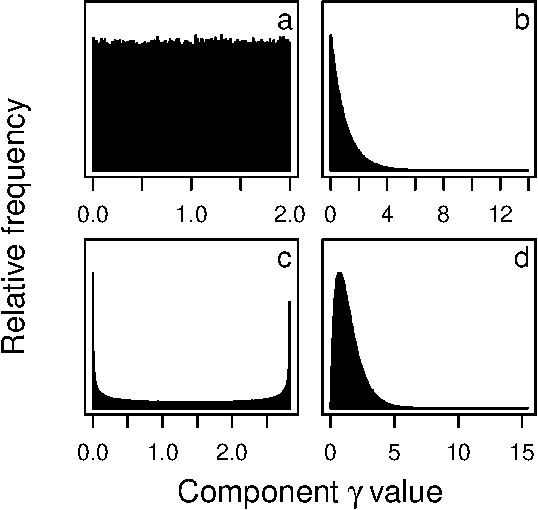
\includegraphics{SI_files/figure-latex/unnamed-chunk-21-1.pdf}

\begin{center}\rule{0.5\linewidth}{\linethickness}\end{center}

The same 100000 \(\mathbf{M}\) matrices were used to investigate
stability when applying each of these different distributions of
\(\gamma\) values. The table below shows the number of \(\mathbf{M}\)
that were unstable (\_unst) and stable (\_stbl) for the exponential
(Exp), beta, and gamma distributions.

\begin{longtable}[]{@{}lllllll@{}}
\toprule
S & Exp\_unst & Exp\_stbl & beta\_unst & beta\_stbl & gamma\_unst &
gamma\_stbl\tabularnewline
\midrule
\endhead
2 & 30 & 99970 & 30 & 99970 & 30 & 99970\tabularnewline
3 & 355 & 99645 & 355 & 99645 & 355 & 99645\tabularnewline
4 & 1506 & 98494 & 1512 & 98488 & 1516 & 98484\tabularnewline
5 & 3930 & 96070 & 3971 & 96029 & 4006 & 95994\tabularnewline
6 & 7738 & 92262 & 7844 & 92156 & 7918 & 92082\tabularnewline
7 & 13606 & 86394 & 13889 & 86111 & 13990 & 86010\tabularnewline
8 & 20535 & 79465 & 21002 & 78998 & 21114 & 78886\tabularnewline
9 & 28614 & 71386 & 29060 & 70940 & 29110 & 70890\tabularnewline
10 & 38375 & 61625 & 38388 & 61612 & 38441 & 61559\tabularnewline
11 & 48616 & 51384 & 48211 & 51789 & 47957 & 52043\tabularnewline
12 & 59254 & 40746 & 58025 & 41975 & 57473 & 42527\tabularnewline
13 & 68816 & 31184 & 66753 & 33247 & 66127 & 33873\tabularnewline
14 & 77721 & 22279 & 75149 & 24851 & 74222 & 25778\tabularnewline
15 & 84842 & 15158 & 82030 & 17970 & 81040 & 18960\tabularnewline
16 & 90365 & 9635 & 87809 & 12191 & 86600 & 13400\tabularnewline
17 & 94171 & 5829 & 91756 & 8244 & 90668 & 9332\tabularnewline
18 & 96978 & 3022 & 94977 & 5023 & 94176 & 5824\tabularnewline
19 & 98376 & 1624 & 97018 & 2982 & 96268 & 3732\tabularnewline
20 & 99218 & 782 & 98357 & 1643 & 97765 & 2235\tabularnewline
21 & 99678 & 322 & 99124 & 876 & 98746 & 1254\tabularnewline
22 & 99864 & 136 & 99599 & 401 & 99323 & 677\tabularnewline
23 & 99954 & 46 & 99783 & 217 & 99668 & 332\tabularnewline
24 & 99978 & 22 & 99920 & 80 & 99821 & 179\tabularnewline
25 & 99996 & 4 & 99967 & 33 & 99911 & 89\tabularnewline
26 & 99999 & 1 & 99979 & 21 & 99960 & 40\tabularnewline
27 & 99999 & 1 & 99990 & 10 & 99983 & 17\tabularnewline
28 & 100000 & 0 & 99999 & 1 & 99991 & 9\tabularnewline
29 & 100000 & 0 & 99999 & 1 & 99999 & 1\tabularnewline
30 & 100000 & 0 & 100000 & 0 & 100000 & 0\tabularnewline
31 & 100000 & 0 & 100000 & 0 & 99999 & 1\tabularnewline
32 & 100000 & 0 & 100000 & 0 & 100000 & 0\tabularnewline
\ldots{} & \ldots{} & \ldots{} & \ldots{} & \ldots{} & \ldots{} &
\ldots{}\tabularnewline
50 & 100000 & 0 & 100000 & 0 & 100000 & 0\tabularnewline
\bottomrule
\end{longtable}

In comparison to the uniform distribution (a), proportionally fewer
random systems are found with the exponential distribution (b), while
more are found with the beta (c) and gamma (d) distributions.

\hypertarget{Feasibility}{\section{Feasibility of complex
systems}\label{Feasibility}}

When feasibility was evaluated with and without variation in \(\gamma\),
there was no increase in stability for \(\mathbf{M}\) where \(\gamma\)
varied as compared to where \(\gamma = 1\). Results below illustrate
this result, which was general to all other simulations performed.

\begin{longtable}[]{@{}rrrrrrr@{}}
\toprule
S & A0\_infeasible & A0\_feasible & A1\_infeasible & A1\_feasible &
A1\_made\_feasible & A1\_made\_infeasible\tabularnewline
\midrule
\endhead
2 & 749978 & 250022 & 749942 & 250058 & 35552 & 35516\tabularnewline
3 & 874519 & 125481 & 874296 & 125704 & 36803 & 36580\tabularnewline
4 & 937192 & 62808 & 937215 & 62785 & 26440 & 26463\tabularnewline
5 & 968776 & 31224 & 968639 & 31361 & 16319 & 16182\tabularnewline
6 & 984313 & 15687 & 984463 & 15537 & 9006 & 9156\tabularnewline
7 & 992149 & 7851 & 992161 & 7839 & 4991 & 5003\tabularnewline
8 & 996124 & 3876 & 996103 & 3897 & 2644 & 2623\tabularnewline
9 & 998014 & 1986 & 998027 & 1973 & 1361 & 1374\tabularnewline
10 & 999031 & 969 & 999040 & 960 & 698 & 707\tabularnewline
11 & 999546 & 454 & 999514 & 486 & 377 & 345\tabularnewline
12 & 999764 & 236 & 999792 & 208 & 160 & 188\tabularnewline
13 & 999883 & 117 & 999865 & 135 & 105 & 87\tabularnewline
14 & 999938 & 62 & 999945 & 55 & 40 & 47\tabularnewline
15 & 999971 & 29 & 999964 & 36 & 31 & 24\tabularnewline
16 & 999988 & 12 & 999991 & 9 & 8 & 11\tabularnewline
17 & 999996 & 4 & 999991 & 9 & 8 & 3\tabularnewline
18 & 999997 & 3 & 999999 & 1 & 1 & 3\tabularnewline
19 & 999998 & 2 & 999997 & 3 & 3 & 2\tabularnewline
20 & 1000000 & 0 & 999999 & 1 & 1 & 0\tabularnewline
21 & 1000000 & 0 & 1000000 & 0 & 0 & 0\tabularnewline
22 & 999999 & 1 & 1000000 & 0 & 0 & 1\tabularnewline
23 & 1000000 & 0 & 1000000 & 0 & 0 & 0\tabularnewline
24 & 1000000 & 0 & 1000000 & 0 & 0 & 0\tabularnewline
25 & 1000000 & 0 & 1000000 & 0 & 0 & 0\tabularnewline
26 & 1000000 & 0 & 1000000 & 0 & 0 & 0\tabularnewline
27 & 1000000 & 0 & 1000000 & 0 & 0 & 0\tabularnewline
28 & 1000000 & 0 & 1000000 & 0 & 0 & 0\tabularnewline
29 & 1000000 & 0 & 1000000 & 0 & 0 & 0\tabularnewline
30 & 1000000 & 0 & 1000000 & 0 & 0 & 0\tabularnewline
31 & 1000000 & 0 & 1000000 & 0 & 0 & 0\tabularnewline
32 & 1000000 & 0 & 1000000 & 0 & 0 & 0\tabularnewline
33 & 1000000 & 0 & 1000000 & 0 & 0 & 0\tabularnewline
34 & 1000000 & 0 & 1000000 & 0 & 0 & 0\tabularnewline
35 & 1000000 & 0 & 1000000 & 0 & 0 & 0\tabularnewline
36 & 1000000 & 0 & 1000000 & 0 & 0 & 0\tabularnewline
37 & 1000000 & 0 & 1000000 & 0 & 0 & 0\tabularnewline
38 & 1000000 & 0 & 1000000 & 0 & 0 & 0\tabularnewline
39 & 1000000 & 0 & 1000000 & 0 & 0 & 0\tabularnewline
40 & 1000000 & 0 & 1000000 & 0 & 0 & 0\tabularnewline
41 & 1000000 & 0 & 1000000 & 0 & 0 & 0\tabularnewline
42 & 1000000 & 0 & 1000000 & 0 & 0 & 0\tabularnewline
43 & 1000000 & 0 & 1000000 & 0 & 0 & 0\tabularnewline
44 & 1000000 & 0 & 1000000 & 0 & 0 & 0\tabularnewline
45 & 1000000 & 0 & 1000000 & 0 & 0 & 0\tabularnewline
46 & 1000000 & 0 & 1000000 & 0 & 0 & 0\tabularnewline
47 & 1000000 & 0 & 1000000 & 0 & 0 & 0\tabularnewline
48 & 1000000 & 0 & 1000000 & 0 & 0 & 0\tabularnewline
49 & 1000000 & 0 & 1000000 & 0 & 0 & 0\tabularnewline
50 & 1000000 & 0 & 1000000 & 0 & 0 & 0\tabularnewline
\bottomrule
\end{longtable}

Hence, in general, \(Var(\gamma)\) does not appear to affect feasibility
in pure species interaction
networks\textsuperscript{\protect\hyperlink{ref-Servan2018}{4}}.

\hypertarget{ga}{\section{\texorpdfstring{Stability given targeted
manipulation of \(\gamma\) (genetic
algorithm)}{Stability given targeted manipulation of \textbackslash{}gamma (genetic algorithm)}}\label{ga}}

The figure below compares the stability of large complex systems given
\(\boldsymbol{\gamma = 1}\) versus targeted manipulation of \(\gamma\)
elements. For each \(S\), 100000 complex systems are randomly generated.
Stability of each complex system is tested given variation in \(\gamma\)
using a genetic algorithm to maximise the effect of \(\gamma\) values on
increasing stability, as compared to stability in an otherwise identical
system in which \(\gamma\) is the same for all components. Blue bars
show the number of stable systems in the absence of component response
rate variation, while red bars show the number of stable systems that
can be generated if component response rate is varied to maximise system
stability. The black line shows the proportion of systems that are
stable when component response rate is targeted to increase stability,
but would not be stable if \(\sigma^{2}_{\gamma} = 0\). The y-axis shows
the \(\ln\) number of systems that are stable across
\(S = \{1, 2, ..., 39, 40\}\) for \(C = 1\), and the proportion of
systems wherein a targeted search of \(\gamma\) values successfully
resulted in system stability.

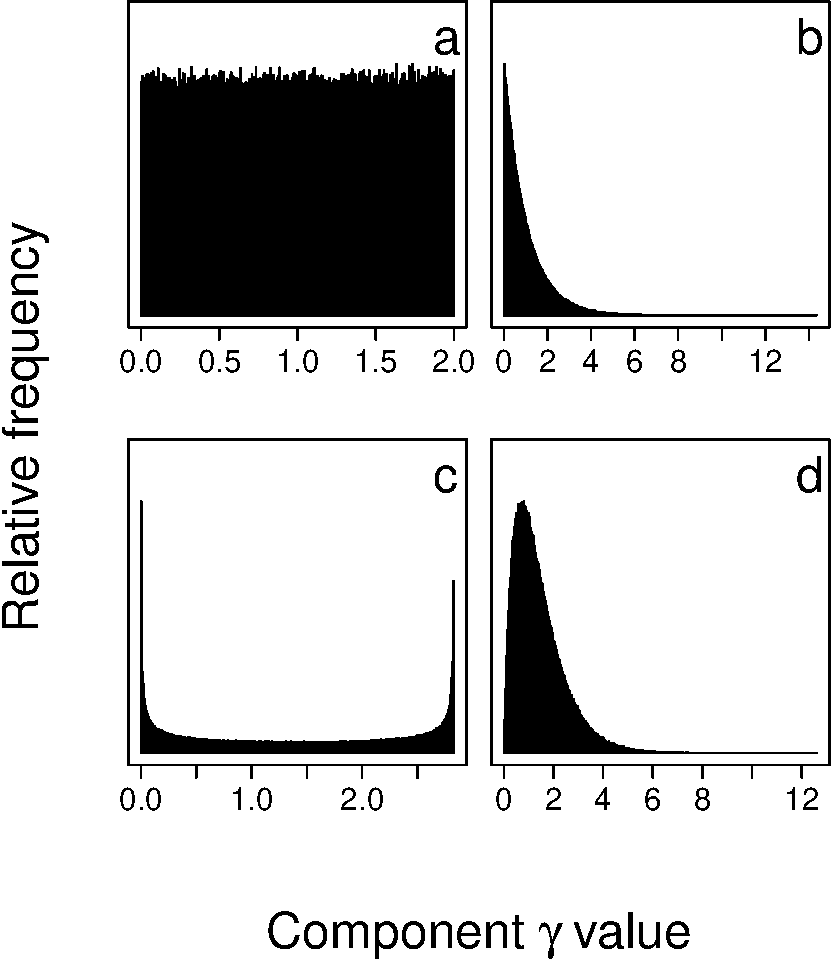
\includegraphics{SI_files/figure-latex/unnamed-chunk-24-1.pdf}

Stability results are also shown in the table below. Results for
\texttt{A0} indicate systems in which \(\gamma = 1\), while \texttt{A1}
refers to systems in which the genetic algorithm searched for a set of
\(\gamma\) values that stabilised the system.

\begin{longtable}[]{@{}rrrrrrr@{}}
\toprule
S & A0\_unstable & A0\_stable & A1\_unstable & A1\_stable &
A1\_stabilised & A1\_destabilised\tabularnewline
\midrule
\endhead
2 & 26 & 99974 & 26 & 99974 & 0 & 0\tabularnewline
3 & 358 & 99642 & 358 & 99642 & 0 & 0\tabularnewline
4 & 1505 & 98495 & 1505 & 98495 & 0 & 0\tabularnewline
5 & 3995 & 96005 & 3982 & 96018 & 13 & 0\tabularnewline
6 & 8060 & 91940 & 7956 & 92044 & 104 & 0\tabularnewline
7 & 13420 & 86580 & 12953 & 87047 & 468 & 1\tabularnewline
8 & 20518 & 79482 & 18940 & 81060 & 1578 & 0\tabularnewline
9 & 28939 & 71061 & 25148 & 74852 & 3793 & 2\tabularnewline
10 & 38241 & 61759 & 30915 & 69085 & 7327 & 1\tabularnewline
11 & 48682 & 51318 & 36398 & 63602 & 12286 & 2\tabularnewline
12 & 58752 & 41248 & 40710 & 59290 & 18043 & 1\tabularnewline
13 & 68888 & 31112 & 44600 & 55400 & 24289 & 1\tabularnewline
14 & 77651 & 22349 & 47528 & 52472 & 30124 & 1\tabularnewline
15 & 84912 & 15088 & 49971 & 50029 & 34942 & 1\tabularnewline
16 & 90451 & 9549 & 52274 & 47726 & 38178 & 1\tabularnewline
17 & 94332 & 5668 & 54124 & 45876 & 40209 & 1\tabularnewline
18 & 96968 & 3032 & 55831 & 44169 & 41139 & 2\tabularnewline
19 & 98384 & 1616 & 58079 & 41921 & 40305 & 0\tabularnewline
20 & 99269 & 731 & 60181 & 39819 & 39088 & 0\tabularnewline
21 & 99677 & 323 & 63338 & 36662 & 36339 & 0\tabularnewline
22 & 99854 & 146 & 66350 & 33650 & 33504 & 0\tabularnewline
23 & 99947 & 53 & 70478 & 29522 & 29469 & 0\tabularnewline
24 & 99983 & 17 & 74121 & 25879 & 25862 & 0\tabularnewline
25 & 99991 & 9 & 78364 & 21636 & 21627 & 0\tabularnewline
26 & 99999 & 1 & 82635 & 17365 & 17364 & 0\tabularnewline
27 & 100000 & 0 & 86433 & 13567 & 13567 & 0\tabularnewline
28 & 100000 & 0 & 89951 & 10049 & 10049 & 0\tabularnewline
29 & 100000 & 0 & 92716 & 7284 & 7284 & 0\tabularnewline
30 & 100000 & 0 & 95171 & 4829 & 4829 & 0\tabularnewline
31 & 100000 & 0 & 96844 & 3156 & 3156 & 0\tabularnewline
32 & 100000 & 0 & 98128 & 1872 & 1872 & 0\tabularnewline
33 & 100000 & 0 & 98941 & 1059 & 1059 & 0\tabularnewline
34 & 100000 & 0 & 99358 & 642 & 642 & 0\tabularnewline
35 & 100000 & 0 & 99702 & 298 & 298 & 0\tabularnewline
36 & 100000 & 0 & 99856 & 144 & 144 & 0\tabularnewline
37 & 100000 & 0 & 99921 & 79 & 79 & 0\tabularnewline
38 & 100000 & 0 & 99970 & 30 & 30 & 0\tabularnewline
39 & 100000 & 0 & 99989 & 11 & 11 & 0\tabularnewline
40 & 100000 & 0 & 99994 & 6 & 6 & 0\tabularnewline
\bottomrule
\end{longtable}

The distributions of nine \(\gamma\) vectors from the highest \(S\)
values are shown below. This comparison shows the high number of stable
\(\mathbf{M}\) that can be produced through a targeted search of
\(\gamma\) values, and suggests that many otherwise unstable systems
could potentially be stabilised by an informed manipulation of their
component response times. Such a possibility might conceivably reduce
the dimensionality of problems involving stability in social-ecological
or economic systems.

Distributions of \(\gamma\) values in vectors for the highest values of
\(S\) are shown below.

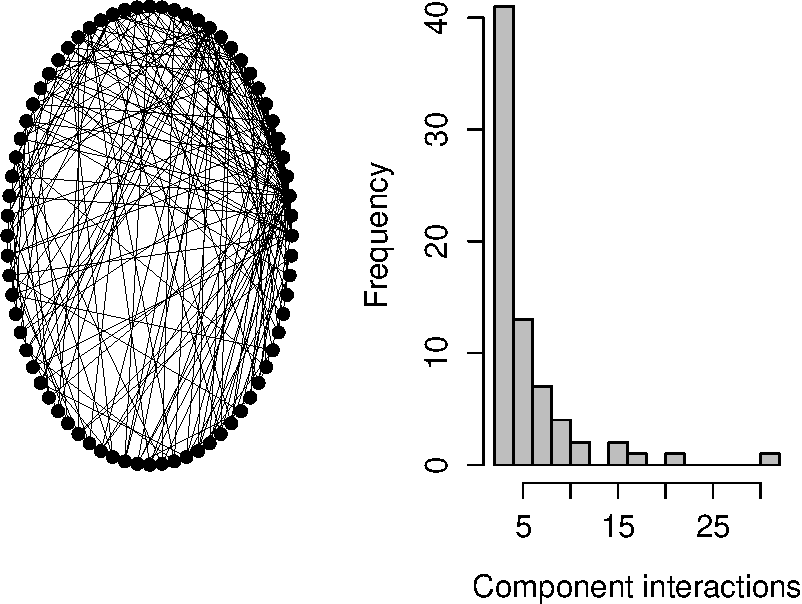
\includegraphics{SI_files/figure-latex/unnamed-chunk-26-1.pdf}

The distribution of \(\gamma\) values found by the genetic algorithm is
uniform. A uniform distribution was used to initialise \(\gamma\)
values, so there is therefore no evidence that a particular distribution
of \(\gamma\) is likely to be found to stabilise a matrix
\(\mathbf{M}\).

\hypertarget{Gibbs}{\section{Consistency with Gibbs et al.
(2018)}\label{Gibbs}}

The question that I address in the main text is distinct from that of
Gibbs et al.\textsuperscript{\protect\hyperlink{ref-Gibbs2017}{5}}, who
focused instead on the effect of a diagonal matrix of biological species
densities \(\mathbf{X}\) on a community matrix \(\mathbf{M}\) given a
species interaction matrix \(\mathbf{A}\). This is modelled as below,

\[\mathbf{M} = \mathbf{XA}.\]

Mathematically, the above is identical to my model in the main text
where the system \(\mathbf{M}\) is defined by component interaction
strengths \(\mathbf{A}\) and individual component response rates
\(\mathbf{\gamma}\),

\[\mathbf{M} = \mathbf{\gamma A}.\]

I focused on the probability of observing a stable versus unstable
system given variation in \(\mathbf{\gamma}\) as system complexity
(\(\sigma\sqrt{SC}\)) increased. I increased system complexity by
holding \(C\) and \(\sigma\) constant and incrementally increasing \(S\)
to obtain numerical results. In contrast, Gibbs et
al.\textsuperscript{\protect\hyperlink{ref-Gibbs2017}{5}} applied
analytical techniques to instead focus on a different question
concerning the effect of \(\mathbf{\gamma}\) on the stability of
\(\mathbf{M}\) given \(\mathbf{A}\) as \(S \to \infty\), with \(\sigma\)
scaled so that \(\sigma = 1/\sqrt{S}\). Under such scaling, Gibbs et
al.\textsuperscript{\protect\hyperlink{ref-Gibbs2017}{5}} showed that
the effect of \(\gamma\) on stability should decrease exponentially as
\(S\) increases, which I demonstrate below by running simulations in
which \(\sigma = 1/\sqrt{S}\).

\begin{longtable}[]{@{}rrrrrrr@{}}
\toprule
N & A0\_unstable & A0\_stable & A1\_unstable & A1\_stable &
A1\_stabilised & A1\_destabilised\tabularnewline
\midrule
\endhead
2 & 3111 & 96889 & 3111 & 96889 & 0 & 0\tabularnewline
3 & 5203 & 94797 & 5237 & 94763 & 1 & 35\tabularnewline
4 & 6743 & 93257 & 6818 & 93182 & 6 & 81\tabularnewline
5 & 7889 & 92111 & 8005 & 91995 & 20 & 136\tabularnewline
6 & 8834 & 91166 & 8991 & 91009 & 55 & 212\tabularnewline
7 & 9885 & 90115 & 10072 & 89928 & 81 & 268\tabularnewline
8 & 10516 & 89484 & 10764 & 89236 & 108 & 356\tabularnewline
9 & 11135 & 88865 & 11383 & 88617 & 145 & 393\tabularnewline
10 & 11819 & 88181 & 12095 & 87905 & 181 & 457\tabularnewline
11 & 12414 & 87586 & 12700 & 87300 & 213 & 499\tabularnewline
12 & 12865 & 87135 & 13136 & 86864 & 283 & 554\tabularnewline
13 & 13530 & 86470 & 13836 & 86164 & 324 & 630\tabularnewline
14 & 13745 & 86255 & 14042 & 85958 & 362 & 659\tabularnewline
15 & 14401 & 85599 & 14720 & 85280 & 387 & 706\tabularnewline
16 & 14793 & 85207 & 15123 & 84877 & 428 & 758\tabularnewline
17 & 15004 & 84996 & 15356 & 84644 & 444 & 796\tabularnewline
18 & 15361 & 84639 & 15735 & 84265 & 472 & 846\tabularnewline
19 & 16062 & 83938 & 16303 & 83697 & 592 & 833\tabularnewline
20 & 15814 & 84186 & 16184 & 83816 & 566 & 936\tabularnewline
21 & 16171 & 83829 & 16492 & 83508 & 640 & 961\tabularnewline
22 & 16671 & 83329 & 17049 & 82951 & 641 & 1019\tabularnewline
23 & 17000 & 83000 & 17291 & 82709 & 718 & 1009\tabularnewline
24 & 17411 & 82589 & 17666 & 82334 & 765 & 1020\tabularnewline
25 & 17414 & 82586 & 17742 & 82258 & 783 & 1111\tabularnewline
26 & 17697 & 82303 & 18027 & 81973 & 806 & 1136\tabularnewline
27 & 18010 & 81990 & 18316 & 81684 & 880 & 1186\tabularnewline
28 & 18584 & 81416 & 18735 & 81265 & 1008 & 1159\tabularnewline
29 & 18401 & 81599 & 18572 & 81428 & 942 & 1113\tabularnewline
30 & 18497 & 81503 & 18754 & 81246 & 952 & 1209\tabularnewline
31 & 18744 & 81256 & 18942 & 81058 & 991 & 1189\tabularnewline
32 & 18936 & 81064 & 19194 & 80806 & 1022 & 1280\tabularnewline
33 & 19174 & 80826 & 19346 & 80654 & 1113 & 1285\tabularnewline
34 & 19477 & 80523 & 19632 & 80368 & 1120 & 1275\tabularnewline
35 & 19659 & 80341 & 19777 & 80223 & 1206 & 1324\tabularnewline
36 & 19883 & 80117 & 19929 & 80071 & 1275 & 1321\tabularnewline
37 & 20275 & 79725 & 20348 & 79652 & 1308 & 1381\tabularnewline
38 & 20067 & 79933 & 20190 & 79810 & 1275 & 1398\tabularnewline
39 & 20416 & 79584 & 20516 & 79484 & 1340 & 1440\tabularnewline
40 & 20370 & 79630 & 20489 & 79511 & 1359 & 1478\tabularnewline
41 & 20295 & 79705 & 20430 & 79570 & 1382 & 1517\tabularnewline
42 & 20767 & 79233 & 20839 & 79161 & 1418 & 1490\tabularnewline
43 & 20688 & 79312 & 20705 & 79295 & 1471 & 1488\tabularnewline
44 & 21049 & 78951 & 21028 & 78972 & 1555 & 1534\tabularnewline
45 & 21114 & 78886 & 21034 & 78966 & 1572 & 1492\tabularnewline
46 & 21163 & 78837 & 21195 & 78805 & 1463 & 1495\tabularnewline
47 & 21373 & 78627 & 21353 & 78647 & 1535 & 1515\tabularnewline
48 & 21338 & 78662 & 21285 & 78715 & 1632 & 1579\tabularnewline
49 & 21547 & 78453 & 21566 & 78434 & 1575 & 1594\tabularnewline
50 & 21738 & 78262 & 21633 & 78367 & 1636 & 1531\tabularnewline
51 & 21967 & 78033 & 21892 & 78108 & 1698 & 1623\tabularnewline
\bottomrule
\end{longtable}

Above table results can be compared to those of the
\protect\hyperlink{IncrS}{main results}. Note that 100000 (not 1
million), simulations are run to confirm consistency with Gibbs et
al.\textsuperscript{\protect\hyperlink{ref-Gibbs2017}{5}}. The
difference between my model and Gibbs et
al.\textsuperscript{\protect\hyperlink{ref-Gibbs2017}{5}} is that in the
latter, \(\sigma\sqrt{SC} = 1\) remains constant with increasing \(S\).
In the former, \(\sigma\sqrt{SC}\) increases with \(S\), so the expected
complexity of the system also increases accordingly. Consequently, for
the scaled \(\sigma\) in the table above, systems are not more likely to
be stabilised by \(\gamma\) as \(S\) increases, consistent with Gibbs et
al.\textsuperscript{\protect\hyperlink{ref-Gibbs2017}{5}}. Note that
overall stability does decrease with increasing \(S\) due to the
increased density of eigenvalues (see below).

\begin{figure}[H]

{\centering 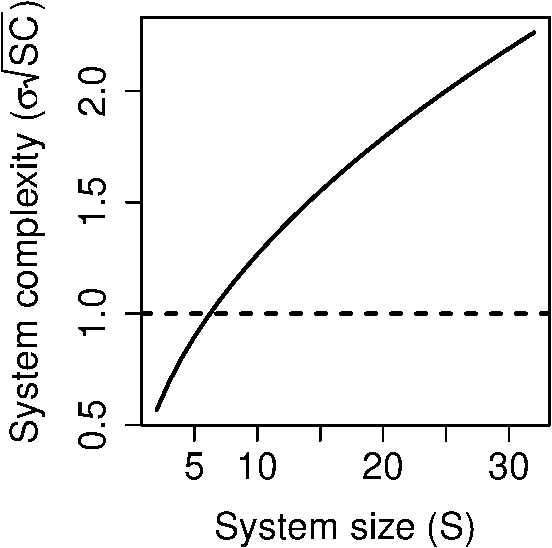
\includegraphics{SI_files/figure-latex/unnamed-chunk-28-1} 

}

\end{figure}

\textbf{Complexity as a function of \(S\) in the main text (solid)
versus in Gibbs et
al.\textsuperscript{\protect\hyperlink{ref-Gibbs2017}{5}} (dashed).}

When the complexity is scaled to \(\sigma\sqrt{SC} = 1\), an increase in
\(S\) increases the eigenvalue density within a circle with a unit
radius centred at \((-1, 0)\) on the complex plane. As \(S \to \infty\),
this circle becomes increasingly saturated. Gibbs et
al.\textsuperscript{\protect\hyperlink{ref-Gibbs2017}{5}} showed that a
diagonal matrix \(\mathbf{\gamma}\) will have an exponentially
decreasing effect on stability with increasing \(S\). Increasing \(S\)
is visualised below, first with a system size \(S = 100\).

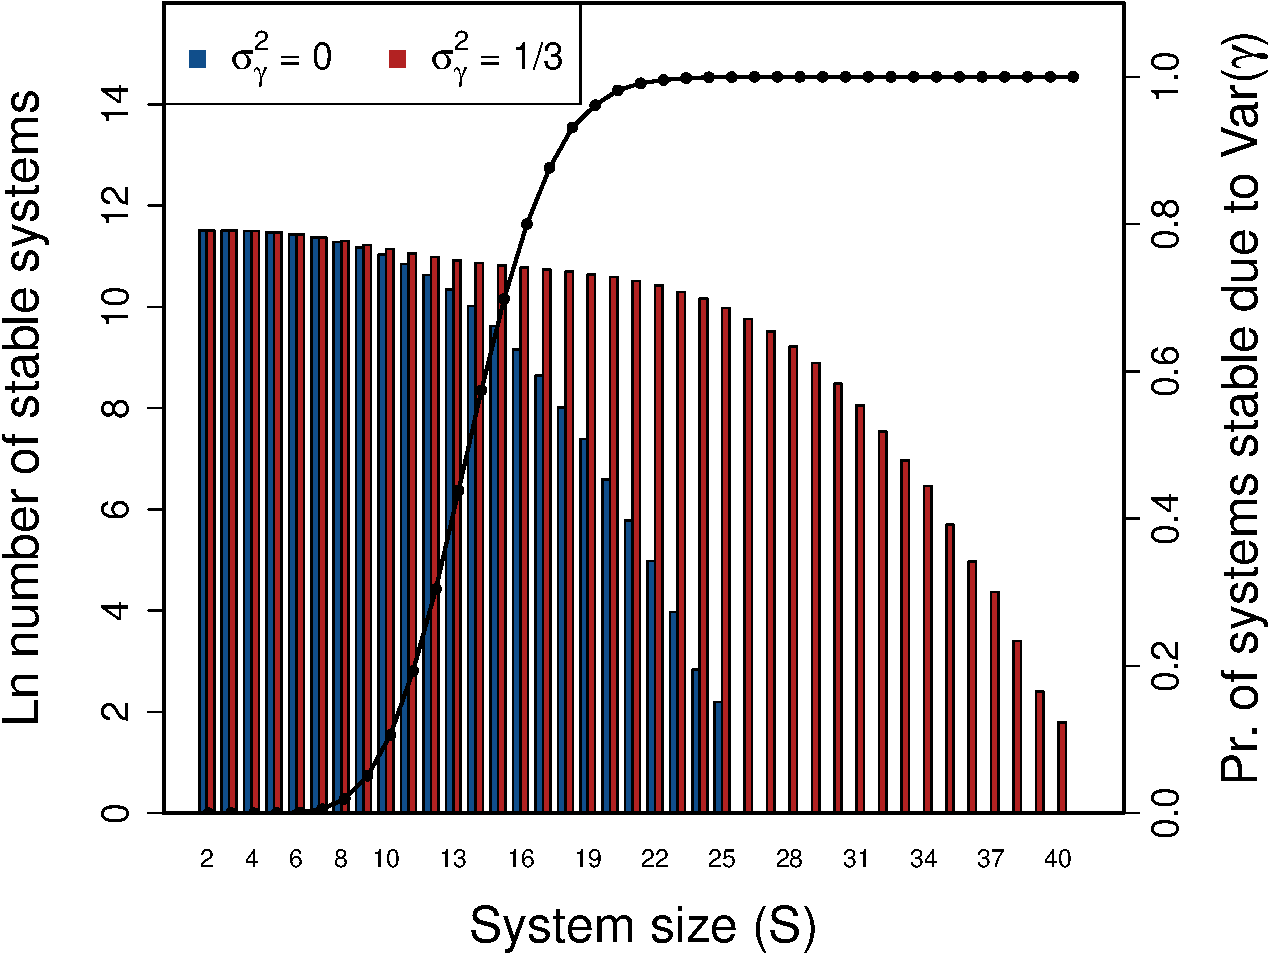
\includegraphics{SI_files/figure-latex/unnamed-chunk-30-1.pdf}

The left panel above shows the distribution of eigenvalues; the blue
ellipse shows the unit radius within which eigenvalues are expected to
be contained. The right panel shows how eigenvalue distributions change
given \(\gamma \sim \mathcal{U}(0,2)\). The vertical dotted line shows
the threshold of stability, \(\Re = 0\). Increasing to \(S = 200\), the
scaling \(\sigma = 1 / \sqrt{S}\) maintains the expected distribution of
eigenvalues but increases eigenvalue density.

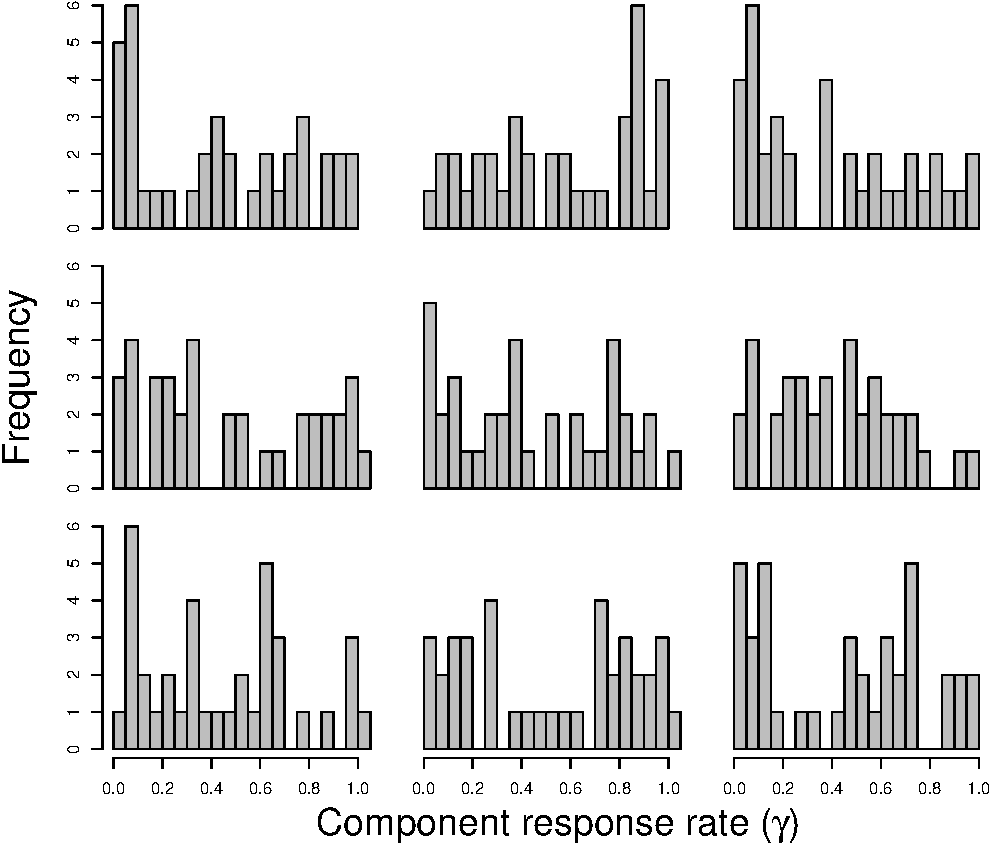
\includegraphics{SI_files/figure-latex/unnamed-chunk-31-1.pdf}

We can increase the system size to \(S = 500\) and see the corresponding
increase in eigenvalue density.

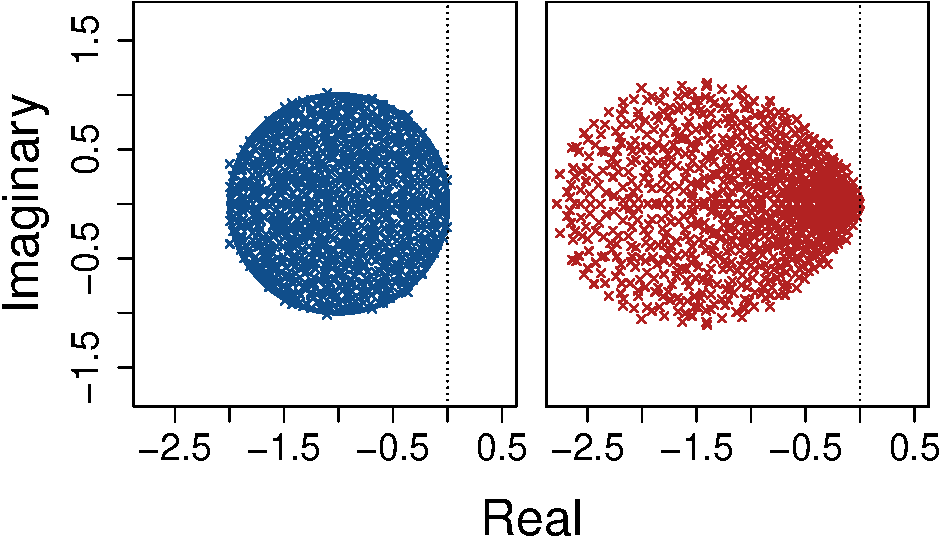
\includegraphics{SI_files/figure-latex/unnamed-chunk-32-1.pdf}

Finally, below shows a increase in system size to \(S = 1000\).

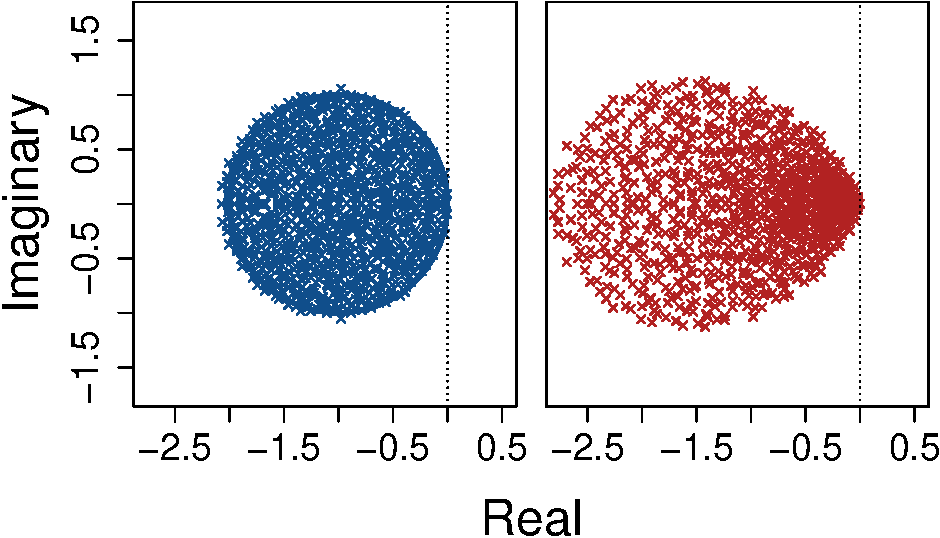
\includegraphics{SI_files/figure-latex/unnamed-chunk-33-1.pdf}

In contrast, in the model of the main text, the complexity of system is
not scaled to \(\sigma\sqrt{SC} = 1\). Rather, the density of
eigenvalues within a circle centred at \((-1, 0)\) with a radius
\(\sigma\sqrt{SC}\) is held constant such that there are
\(S / \pi(\sigma\sqrt{SC})^2\) eigenvalues per unit area of the circle.
As \(S\) increases, so does the expected complexity of the system, but
the density of eigenvalues remains finite causing error around this
expectation. Below shows a system where \(S = 100\), \(C = 0.0625\), and
\(\sigma = 0.4\), where \(\sigma \sqrt{SC} = 1\) (identical to the first
example distribution above in which \(S = 100\) and
\(\sigma = 1/\sqrt{S}\)).

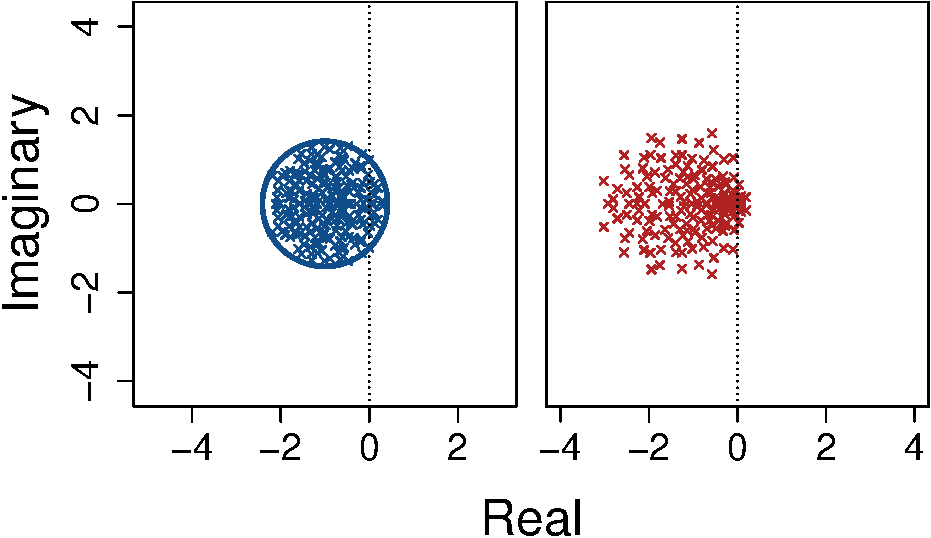
\includegraphics{SI_files/figure-latex/unnamed-chunk-35-1.pdf}

Now when \(S\) is increased to \(200\) while keeping \(C = 0.0625\) and
\(\sigma = 0.4\), the area of the circle within which eigenvalues are
contained increases to keep the density of eigenvalues constant.

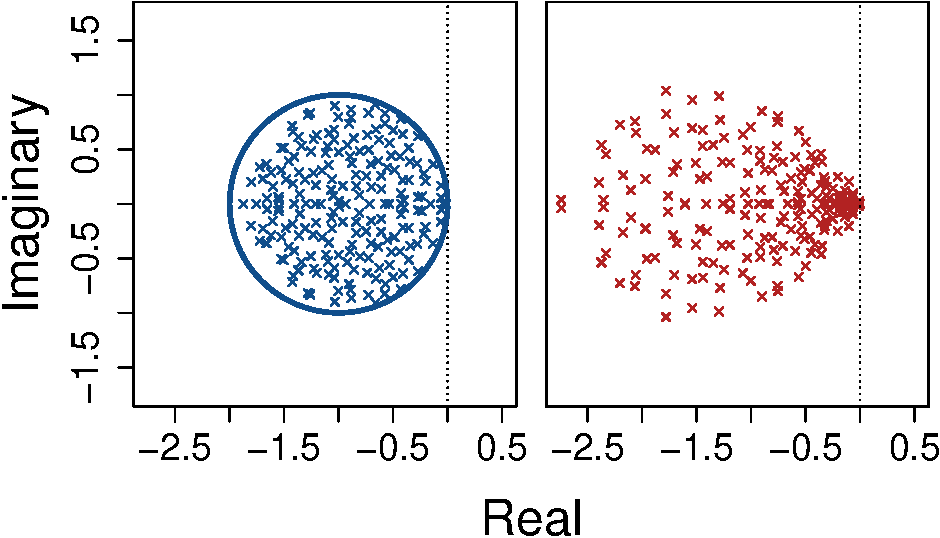
\includegraphics{SI_files/figure-latex/unnamed-chunk-36-1.pdf}

Note that the expected distribution of eigenvalues increases so that the
threshold \(\Re = 0\) is exceeded. Below, system size is increased to
\(S = 500\).

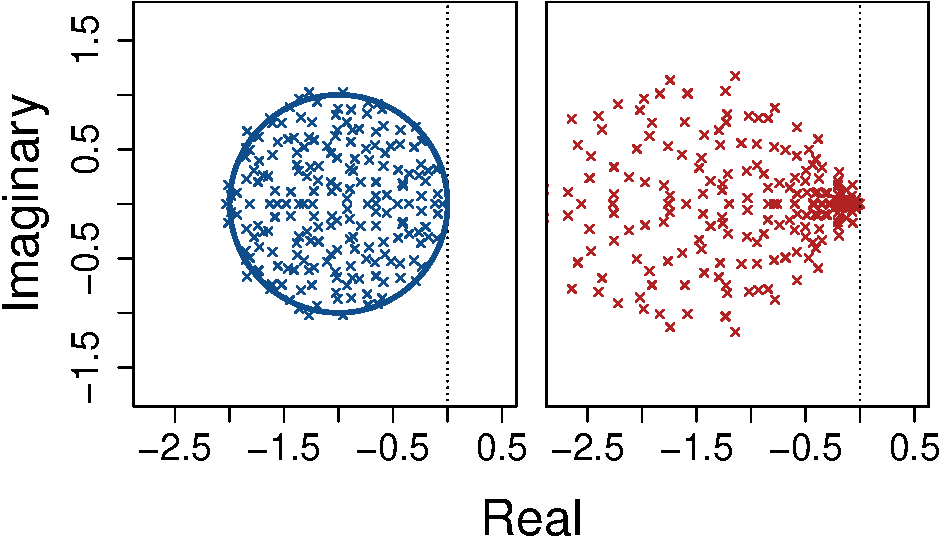
\includegraphics{SI_files/figure-latex/unnamed-chunk-37-1.pdf}

Finally, \(S = 1000\) is shown below. Again, the density of eigenvalues
per unit remains constant at ca 2, but the system has increased in
complexity such that some real components of eigenvalues are almost
assured to be greater than zero.

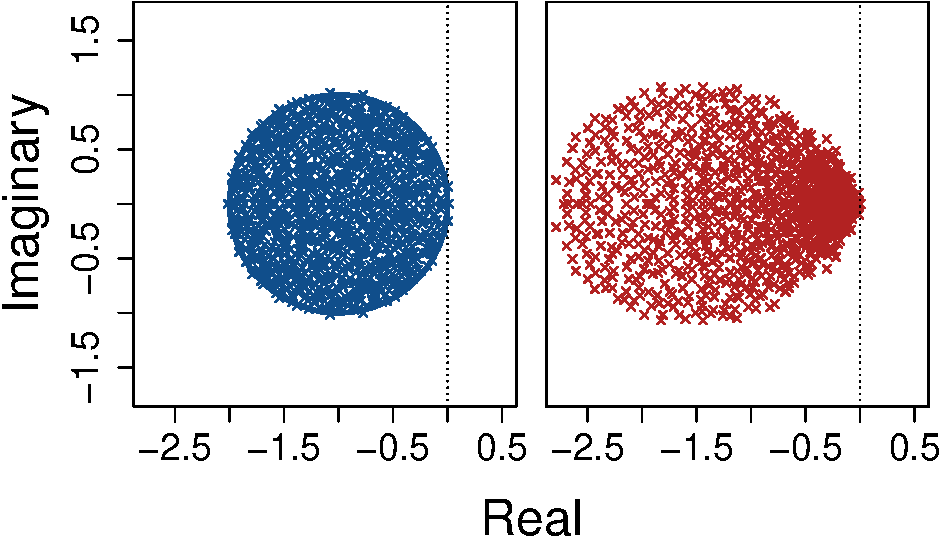
\includegraphics{SI_files/figure-latex/unnamed-chunk-38-1.pdf}

\section{Effects of matrix
correlations}\label{effects-of-matrix-correlations}

\section*{References}\label{references}
\addcontentsline{toc}{section}{References}

\hypertarget{refs}{}
\hypertarget{ref-May1972}{}
1. May, R. M. Will a large complex system be stable? \emph{Nature}
\textbf{238,} 413--414 (1972).

\hypertarget{ref-Allesina2012}{}
2. Allesina, S. \& Tang, S. Stability criteria for complex ecosystems.
\emph{Nature} \textbf{483,} 205--208 (2012).

\hypertarget{ref-Allesina2015}{}
3. Allesina, S. \emph{et al.} Predicting the stability of large
structured food webs. \emph{Nature Communications} \textbf{6,} 7842
(2015).

\hypertarget{ref-Servan2018}{}
4. Serván, C. A., Capitán, J. A., Grilli, J., Morrison, K. E. \&
Allesina, S. Coexistence of many species in random ecosystems.
\emph{Nature Ecology and Evolution} \textbf{2,} 1237--1242 (2018).

\hypertarget{ref-Gibbs2017}{}
5. Gibbs, T., Grilli, J., Rogers, T. \& Allesina, S. The effect of
population abundances on the stability of large random ecosystems.
\emph{Physical Review E - Statistical, Nonlinear, and Soft Matter
Physics} \textbf{98,} 022410 (2018).


\end{document}
